\documentclass{article}
\usepackage[utf8]{inputenc}
\usepackage{geometry}
\usepackage{graphicx}
\usepackage{amsmath}
\usepackage{amsfonts}
\usepackage{amsthm}
\usepackage{amssymb}
\usepackage[most]{tcolorbox}
\usepackage{array}
\usepackage{latexsym}
\usepackage{alltt}
\usepackage{hyperref}
\usepackage{color}
\usepackage{float}
\usepackage{pdfpages}
\usepackage{algpseudocode}
\usepackage{multicol}
\usepackage{multirow}
\usepackage{caption}
\usepackage{xparse}
\usepackage{setspace}
\usepackage{enumitem}


\geometry
{
    a4paper,
    left=10mm,
    right=10mm,
    top=10mm,
    bottom=12mm,
}

% mybox
\newtcolorbox{mybox}[3][]
{
  colframe = #2!25,
  colback  = #2!10,
  coltitle = #2!20!black,  
  title    = {#3},
  #1,
}

% New environments that use mybox
\newcounter{example}
\newenvironment{example}[1]{\begin{mybox}{green}{\refstepcounter{example}\textbf{Example~\theexample #1}}}{\end{mybox}}

\newenvironment{example_break}[1]{\begin{mybox}[breakable]{green}{\refstepcounter{example}\textbf{Example~\theexample #1}}}{\end{mybox}}

\newcounter{definition}
\newenvironment{definition}[1]{\refstepcounter{definition}\begin{mybox}{blue}{\textbf{Definition~\thedefinition #1}}}{\end{mybox}}

\newcounter{theorem}
\newenvironment{theorem}[1]{\begin{mybox}{red}{\refstepcounter{theorem}\textbf{Theorem~\thetheorem #1}}}{\end{mybox}}

\newenvironment{formula}[1]{\begin{mybox}{cyan}{\textbf{#1}}}{\end{mybox}}

% Changing maketitle
\makeatletter         
\renewcommand\maketitle{
{\raggedright % Note the extra {
\begin{center}
{\Large \bfseries \@title}\\[2ex] 
{\large \@author \ - \@date}\\[2ex]
\end{center}}} % Note the extra }
\makeatother

% \onehalfspacing % adjust spacing
\setlength{\parskip}{0.5\baselineskip}

% macros
\newcommand{\prob}[1]{\textbf{\textit{P}}\left\{#1\right\}}
\newcommand{\expc}[1]{\mathbf{E}\left(#1\right)}
\newcommand{\expcs}[1]{\mathbf{E}^2\left(#1\right)}
\newcommand{\var}[1]{\text{Var}\left( #1 \right)}
\newcommand{\std}[1]{\text{Std}\left( #1 \right)}

\NewDocumentCommand{\dsum}{%
    e{^_}
}{%
  {% 
    \displaystyle\sum
    \IfValueT{#1}{^{#1}}
    \IfValueT{#2}{_{#2}}
  }
}%

% maketitle variables
\title{CENG 222 - Cheatsheet}
\author{Burak Metehan Tunçel}
\date{April 2022}

\begin{document}

\maketitle

% \setcounter{section}{1}

\newpage
\section{Chapter 2}

\begin{multicols}{2}
\setlength{\columnsep}{1.5cm}
\setlength{\columnseprule}{0.2pt}

\subsection{DFA: Deterministic Finite Automata}

\begin{definition}{}
  A \textbf{deterministic finite automaton} is a quintuple $M = (K, \Sigma, \delta, s, F)$ where
  \begin{itemize}
    \item $K$ is a finite set of \textbf{states}
    \item $\Sigma$ is an alphabet,
    \item $s \in K$ is the \textbf{initial state}
    \item $F \subseteq K$ is the set of \textbf{final states}
    \item $\delta$, the \textbf{transition function}, is a function from $K \times \Sigma$ to $K$. 
  \end{itemize}
\end{definition}

The \textbf{configuration} of the machine is the \textit{current state and the unread part of the input string}, i.e., a configuration is an element of $K \times \Sigma^*$.

Let $(q, w)$ and $(q',w')$ be two configurations of $M$. Then $(q, w) \vdash_M (q', w')$ if and only if $w = aw'$ for some $a \in \Sigma$ and $q' = \delta(q, a)$. For example, $(q, aabb) \vdash_M (q', abb)$ where $q' = \delta(q, a)$.

$(q, w) \vdash_M (q', w')$ reads $(q, w)$ \textbf{yields} $(q', w')$ in \textbf{one step}. $\vdash^*_M$ is the \textbf{reflexive transitive closure} of $\vdash_M$ (It can be though like the multiple steps). A string $w \in \Sigma^*$ is \textbf{accepted} by $M$ if and only if $(s, w) \vdash^*_M (f, e)$ for some $f \in F$. The \textbf{language} of $M$, $L(M)$, is the set of strings \textit{accepted} by $M$.

\vfill\null
\columnbreak


\subsection{NFA: Nondeterministic Finite Automata}

\begin{definition}{}
  A \textbf{nondeterministic finite automaton} is a quintuple $M = (K, \Sigma, \Delta, s, F)$, where
  \begin{itemize}
    \item $K$ is a finite set of \textbf{states}
    \item $\Sigma$ is an alphabet
    \item $s \in K$ is the \textbf{initial state}
    \item $F \subseteq K$ is the set of \textbf{final states}, and
    \item $\Delta$, the \textbf{transition relation}, is a subset of $K \times (\Sigma \cup \{e\}) \times K$ 
\end{itemize}
\end{definition}

$(q, a, p) \in \Delta$ is called a \textbf{transition} of $M$. $(q, e, p)$ indicates that the machine can pass to state $p$ from state $q$ without reading an input symbol.

The \textbf{configuration} of the machine is the current state and the unread part of the input string, i.e., a configuration is an element of $K \times \Sigma^*$.

Let $(q, w)$ and $(q', w')$ be two configurations of $M$. Then $(q, w) \vdash_M (q', w')$ if and only if $w = aw'$ for some $a \in \Sigma \cup \{e\}$ and $(q, a, q') \in \Delta$.

$(q, w) \vdash_M (q', w')$ reads $(q, w)$ \textbf{yields} $(q', w')$ \textbf{in one step}. $\vdash^*_M$ is the \textbf{reflexive transitive closure} of $\vdash_M$. $(q, w) \vdash^*_M (q', w')$ reads $(q, w)$ yields $(q', w')$. A string $w \in \Sigma^*$ is \textbf{accepted} by $M$ if and only if there is a state $f \in F$ such that $(s, w) \vdash^*_M (f, e)$. The \textbf{language} of $M$, $L(M)$, is the set of strings accepted by $M$.

\textit{A deterministic finite state automaton is just a special type of nondeterministic finite state automaton}. We obtain a DFA when $\Delta$ defines a function from $K \times \Sigma$ to $K$. In other words, an NFA $M = (K, \Sigma, \Delta, s, F)$ is deterministic if there are no transitions of the form $(q, e, p)$ and for each $q \in K$ and $a \in \Sigma$, there exists \textit{exactly one} $p \in K$ such that $(q, a, p) \in \Delta$.

A nondeterministic finite automaton can always be converted to an \textit{equivalent} deterministic finite state automaton.

\begin{theorem}{}
  For each nondeterministic finite automaton, there exists an equivalent deterministic finite automaton.
\end{theorem}

Proof of the theorem is constructive. In proof, one can use subset construction algorithm to construct a DFA from anNFA and then show they are equivalent.

Two automaton (DFA or NFA, one can be DFA and the other can be NFA) $M_1$ and $M_2$ are said to be \textbf{equivalent} when $L(M_1) = L(M_2)$.

\end{multicols}

\newpage
\subsubsection{Subset Construction}

In here, the following is main and formal definition.

\begin{formula}{}
Given an NFA $M = (K, \Sigma, \Delta, s, F)$, the algorithm constructs an equivalent DFA $M' = (K', \Sigma, \delta, s', F')$ as follows. For each state $q \in K$, the set of states that can be reached without reading an input symbol is defined as
  \begin{align*}
    E(q) = \left\{ p \in K\ |\ (q, e) \vdash^*_M (p, e) \right\}
  \end{align*}
  Essentially, $E(q)$ is the reflexive transitive closure of the set $\left\{ q \right\}$ under the relation $\left\{(p, r)\ |\ (p, e, r) \in \Delta \right\}$. The DFA is defined as:
  \begin{align*}
    K' &= 2^K\\
    s' &= E(s)\\
    F' &= \left\{ Q \subseteq K\ |\ Q \cap F \neq \emptyset \right\}\\
    \delta'(Q, a) &= \left\{ E(p) : p \in K, (q, a, p) \in \Delta \textnormal{ for some } q \in Q \right\} \textnormal{ for each $Q \in K'$ and $a \in \Sigma$}\\
    &= \bigcup \left\{ E(p) : p \in K, (q, a, p) \in \Delta \textnormal{ for some } q \in Q \right\}
  \end{align*}
\end{formula}

\begin{multicols}{2}
\setlength{\columnsep}{1.5cm}
\setlength{\columnseprule}{0.2pt}

\begin{equation*}
  E(q) = \left\{ q \right\} \cup \left\{ p \in K\ |\ (q, e) \vdash^*_M (p, e) \right\}
\end{equation*}

If there is question about transforming an NFA to a DFA, the following steps can be used in question solving:
\begin{formula}{}
  \begin{enumerate}
    \item The NFA $M = (K, \Sigma, \Delta, s, F)$ is given and we want to construct DFA. In other words we want to acquire:
    \begin{equation*}
        M' = (K', \Sigma, \delta', s', F')
    \end{equation*}
    
    \item Start from the initial state of NFA, $s' = E(s)$. For each $q_j \in E(s)$ find the transition for each $k \in \Sigma$ ($q_j, k, q_l$).

    For example, if $E(s) = \{ q_{0}, q_{1} \}$. Look the transition from $q_0$ and $q_1$. If $\Sigma = \{ a, b \}$, then look for $a$ and $b$.
    
    
    \item Then calculate the union of $E(q_i)$ of the reachable states from the state we consider.
    
    For example, if transitions for $a$ are $(q_{0}, a, q_{1}), (q_{1}, a, q_{2})$, then write 
    \begin{quote}
      $(q_{0}, a, q_{1}), (q_{1}, a, q_{2})$ are all the transitions $(q, a, p)$ for some $q \in E(s)$
    \end{quote}
    and calculate the $\delta'(s', a) = E(q_{1}) \cup E(q_{2})$. If it is new state, write this new state on DFA, if not connect it the old one.
    
    \item Follow this steps for each $k \in \Sigma$ and newly introduced steps.
  \end{enumerate}
\end{formula}

\vfill\null
\columnbreak

Look at the example below, it is taken from 2.2.4 in the textbook.

\begin{example}{: NFA to DFA}
  For this example:
  \begin{itemize}
    \item $E(q_0) = \left\{ q_0, q_1, q_2, q_3  \right\}$
    \item $E(q_1) = \left\{ {q_1, q_2, q_3} \right\}$
    \item $E(q_2) = \left\{ q_2 \right\}$
    \item $E(q_3) = \left\{ q_3 \right\}$
    \item $E(q_4) = \left\{ q_3, q_4 \right\}$
  \end{itemize}
  
  \hfill\break

  $s' = E(q_0) = \left\{ q_0, q_1, q_2, q_3  \right\}$,
  \begin{equation*}
    (q_1, a, q_0),\ (q_1, a, q_4), \textnormal{ and } (q_3, a, q_4)
  \end{equation*}
  are all the transitions $(q, a, p)$ for some $q \in s'$. It follows that (Instead of $s'$ any state symbol can be used such as $q_{100}$)
  \begin{equation*}
    \delta'(s', a) = E(q_0) \cup E(q_4) = \left\{ q_0, q_1, q_2, q_3, q_4 \right\}
  \end{equation*}
  Similarly,
  \begin{equation*}
    (q_0, b, q_2) \textnormal{ and } (q_2, b, q_4)
  \end{equation*}
  are all the transitions of the form $(q, b, p)$ for some $q \in E(q_0)$, so
  \begin{equation*}
    \delta'(s', b) = E(q_2) \cup E(q_4) = \left\{ q_2, q_3, q_4 \right\}
  \end{equation*}
  
  In here $\left\{ q_0, q_1, q_2, q_3, q_4 \right\}$ and $\left\{ q_2, q_3, q_4 \right\}$ are new states.
  
  Repeat this calculation for the newly introduced states. In the end, there will be no new states or you will be in wrong way.
\end{example}


\subsection{Finite Automata and Regular Expressions}

\begin{theorem}{}
  The class of languages accepted by finite automata is closed under
  \begin{enumerate}[label=\alph*)]
    \item union
    \item concatenation
    \item Kleene star
    \item complementation
    \item intersection
  \end{enumerate}
\end{theorem}

Let $M_1 = (K_1, \Sigma, \Delta_1, s_1, F_1)$ and $M_2 = (K_2, \Sigma, \Delta_2, s_2, F_2)$ be nondeterministic finite automata.

\begin{enumerate}[label=(\alph*)]
  % (a) Union
  \item \textit{Union.}
  $L(M) = L(M_1) \cup L(M_2)$.
  
  $M = (K, \Sigma, \Delta, s, F)$, where $s$ is a new state not in $K_1$ or $K_2$,
  \begin{itemize}
    \item $K = K_1 \cup K_2 \cup \left\{ s \right\}$
    \item $F = F_1 \cup F_2$
    \item $\Delta = \Delta_1 \cup \Delta_2 \cup \left\{ (s,e,s_1),(s,e,s_2) \right\}$
  \end{itemize}

  % (b) Concatenation
  \item \textit{Concatenation.}
  $L(M) = L(M_1) L(M_2)$.

  Then the finite automaton $M$ that accepts $L(M_1) L(M_2)$ is defined as follows (\textit{May include mistakes}). $M = (K, \Sigma, \Delta, s, F)$
  \begin{itemize}
    \item $s = s_1$
    \item $K = K_1 \cup K_2$
    \item $F = F_2$
    \item $\Delta = \Delta_1 \cup \Delta_2 \cup \left\{ (f,e,s_2)\ |\ f \in F_1 \right\}$
  \end{itemize}

  % (c) Kleenestar
  \item \textit{Kleene star.}
  $L(M) = L(M_1)^*$. 

  Then the finite automaton $M$ that accepts $L(M_1)^*$ is defined as follows (\textit{May include mistakes}). $M = (K, \Sigma, \Delta, s, F)$, where $s$ is not in $M_1$
  \begin{itemize}
    \item $K = K_1 \cup \left\{ s \right\}$
    \item $F = F_1 \cup \left\{ s \right\}$
    \item $\Delta = \Delta_1 \cup \left\{ (s,e,s_1) \right\}$
  \end{itemize}

  % (d) Complementation
  \item \textit{Complementation.}
  $\overline{L} = \Sigma^* - L(M)$. $\overline{M}$ is identical to $M$ except that final and non final states are interchanged.

  $M = (K, \Sigma, \Delta, s, F)$.
  \begin{itemize}
    \item $s = s_1$
    \item $K = K_1$
    \item $F = K \setminus F_1$
    \item $\Delta = \Delta_1$
  \end{itemize}

  % (e) Intersection
  \item \textit{Intersection.}
  \begin{equation*}
    L(M) = L(M_1) \cap L(M_2) = \overline{\overline{L(M_1)} \cup \overline{L(M_2)}}
  \end{equation*}
\end{enumerate}

% \vfill\null
% \columnbreak

\begin{theorem}{}
  \textit{A language is regular if and only if it is accepted by a finite automaton.}
\end{theorem}

\subsubsection{Converting FA to RE}

There are two popular methods for converting a DFA to its regular expression:
\begin{itemize}
  \item Arden's Method
  \item State elimination method
\end{itemize}
Arden's Method is a little more complicated. Consider the state elimination method to convert FA to RE.

\paragraph{Rules}

The rules for state elimination method are as follows
\begin{enumerate}
  \item \textit{The initial state of FA must not have any incoming edge.}

    If there is any incoming edge to the initial edge, then create a new initial state having no incoming edge to it.
  
  \item \textit{There must exist only one final state in FA.}
  
    If there exist multiple final states, then convert all the final states into non-final states and create a new single final state.
  
  \item \textit{The final state of DFA must not have any outgoing edge.}
  
    If this exists, then create a new final state having no outgoing edge from it.
  
  \item \textit{Eliminate all intermediate states one by one.}
\end{enumerate}

% \vfill\null
% \columnbreak

\begin{examplebreak}{}
  Get the regular expression from the following FA:
  \begin{center}
    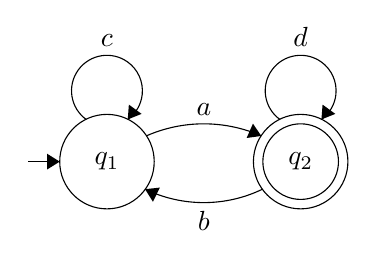
\begin{tikzpicture}[scale=0.2]
    \tikzstyle{every node}+=[inner sep=0pt]
    \draw [black] (5.2,-9.1) circle (3);
    \draw (5.2,-9.1) node {$q_1$};
    \draw [black] (17.5,-9.1) circle (3);
    \draw (17.5,-9.1) node {$q_2$};
    \draw [black] (17.5,-9.1) circle (2.4);
    \draw [black] (0.2,-9.1) -- (2.2,-9.1);
    \fill [black] (2.2,-9.1) -- (1.4,-8.6) -- (1.4,-9.6);
    \draw [black] (7.7,-7.466) arc (113.70628:66.29372:9.079);
    \fill [black] (15,-7.47) -- (14.47,-6.69) -- (14.07,-7.6);
    \draw (11.35,-6.2) node [above] {$a$};
    \draw [black] (15.081,-10.848) arc (-64.17666:-115.82334:8.565);
    \fill [black] (7.62,-10.85) -- (8.12,-11.65) -- (8.56,-10.75);
    \draw (11.35,-12.2) node [below] {$b$};
    \draw [black] (3.877,-6.42) arc (234:-54:2.25);
    \draw (5.2,-1.85) node [above] {$c$};
    \fill [black] (6.52,-6.42) -- (7.4,-6.07) -- (6.59,-5.48);
    \draw [black] (16.177,-6.42) arc (234:-54:2.25);
    \draw (17.5,-1.85) node [above] {$d$};
    \fill [black] (18.82,-6.42) -- (19.7,-6.07) -- (18.89,-5.48);
    \end{tikzpicture}
  \end{center}
  
  \textbf{Step 1:}
    
  Initial state $q_1$ has an incoming edge so create a new initial state $q_i$.
  \begin{center}
    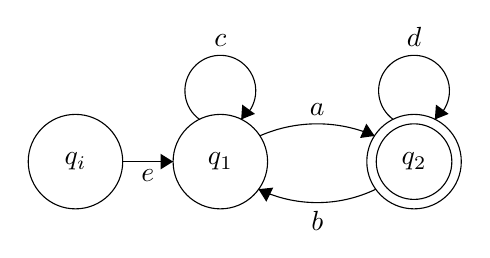
\begin{tikzpicture}[scale=0.2]
    \tikzstyle{every node}+=[inner sep=0pt]
    \draw [black] (12.4,-9.1) circle (3);
    \draw (12.4,-9.1) node {$q_1$};
    \draw [black] (24.7,-9.1) circle (3);
    \draw (24.7,-9.1) node {$q_2$};
    \draw [black] (24.7,-9.1) circle (2.4);
    \draw [black] (3.2,-9.1) circle (3);
    \draw (3.2,-9.1) node {$q_i$};
    \draw [black] (14.9,-7.466) arc (113.70628:66.29372:9.079);
    \fill [black] (22.2,-7.47) -- (21.67,-6.69) -- (21.27,-7.6);
    \draw (18.55,-6.2) node [above] {$a$};
    \draw [black] (22.281,-10.848) arc (-64.17666:-115.82334:8.565);
    \fill [black] (14.82,-10.85) -- (15.32,-11.65) -- (15.76,-10.75);
    \draw (18.55,-12.2) node [below] {$b$};
    \draw [black] (11.077,-6.42) arc (234:-54:2.25);
    \draw (12.4,-1.85) node [above] {$c$};
    \fill [black] (13.72,-6.42) -- (14.6,-6.07) -- (13.79,-5.48);
    \draw [black] (23.377,-6.42) arc (234:-54:2.25);
    \draw (24.7,-1.85) node [above] {$d$};
    \fill [black] (26.02,-6.42) -- (26.9,-6.07) -- (26.09,-5.48);
    \draw [black] (6.2,-9.1) -- (9.4,-9.1);
    \fill [black] (9.4,-9.1) -- (8.6,-8.6) -- (8.6,-9.6);
    \draw (7.8,-9.6) node [below] {$e$};
    \end{tikzpicture}
  \end{center}
  
  \textbf{Step 2:}
  
  Final state $q_2$ has an outgoing edge. So, create a new final state $q_f$.

  \begin{center}
    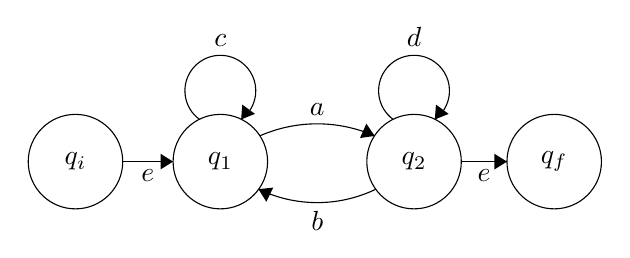
\begin{tikzpicture}[scale=0.2]
    \tikzstyle{every node}+=[inner sep=0pt]
    \draw [black] (12.4,-9.1) circle (3);
    \draw (12.4,-9.1) node {$q_1$};
    \draw [black] (24.7,-9.1) circle (3);
    \draw (24.7,-9.1) node {$q_2$};
    \draw [black] (3.2,-9.1) circle (3);
    \draw (3.2,-9.1) node {$q_i$};
    \draw [black] (33.6,-9.1) circle (3);
    \draw (33.6,-9.1) node {$q_f$};
    \draw [black] (14.9,-7.466) arc (113.70628:66.29372:9.079);
    \fill [black] (22.2,-7.47) -- (21.67,-6.69) -- (21.27,-7.6);
    \draw (18.55,-6.2) node [above] {$a$};
    \draw [black] (22.281,-10.848) arc (-64.17666:-115.82334:8.565);
    \fill [black] (14.82,-10.85) -- (15.32,-11.65) -- (15.76,-10.75);
    \draw (18.55,-12.2) node [below] {$b$};
    \draw [black] (11.077,-6.42) arc (234:-54:2.25);
    \draw (12.4,-1.85) node [above] {$c$};
    \fill [black] (13.72,-6.42) -- (14.6,-6.07) -- (13.79,-5.48);
    \draw [black] (23.377,-6.42) arc (234:-54:2.25);
    \draw (24.7,-1.85) node [above] {$d$};
    \fill [black] (26.02,-6.42) -- (26.9,-6.07) -- (26.09,-5.48);
    \draw [black] (6.2,-9.1) -- (9.4,-9.1);
    \fill [black] (9.4,-9.1) -- (8.6,-8.6) -- (8.6,-9.6);
    \draw (7.8,-9.6) node [below] {$e$};
    \draw [black] (27.7,-9.1) -- (30.6,-9.1);
    \fill [black] (30.6,-9.1) -- (29.8,-8.6) -- (29.8,-9.6);
    \draw (29.15,-9.6) node [below] {$e$};
    \end{tikzpicture}
  \end{center}

  \textbf{Step 3:}

  Start eliminating intermediate states

  \textbf{First eliminate $q_1$:}

  \quad There is a path going from $q_i$ to $q_2$ via $q_1$. So, after eliminating $q_1$ we can connect a direct path from $q_i$ to $q_2$ having cost: $e c^* a = c^* a$.

  \quad There is a loop on $q_2$ using state $q_i$. So, after eliminating $q_1$ we put a direct loop to $q_2$ having cost: $b c^* a$.

  After eliminating $q_1$, the FA looks like following
  \begin{center}
    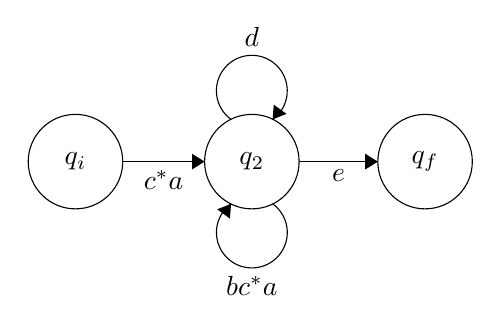
\begin{tikzpicture}[scale=0.2]
    \tikzstyle{every node}+=[inner sep=0pt]
    \draw [black] (14.4,-9.1) circle (3);
    \draw (14.4,-9.1) node {$q_2$};
    \draw [black] (3.2,-9.1) circle (3);
    \draw (3.2,-9.1) node {$q_i$};
    \draw [black] (25.4,-9.1) circle (3);
    \draw (25.4,-9.1) node {$q_f$};
    \draw [black] (13.077,-6.42) arc (234:-54:2.25);
    \draw (14.4,-1.85) node [above] {$d$};
    \fill [black] (15.72,-6.42) -- (16.6,-6.07) -- (15.79,-5.48);
    \draw [black] (17.4,-9.1) -- (22.4,-9.1);
    \fill [black] (22.4,-9.1) -- (21.6,-8.6) -- (21.6,-9.6);
    \draw (19.9,-9.6) node [below] {$e$};
    \draw [black] (6.2,-9.1) -- (11.4,-9.1);
    \fill [black] (11.4,-9.1) -- (10.6,-8.6) -- (10.6,-9.6);
    \draw (8.8,-9.6) node [below] {$c^*a$};
    \draw [black] (15.723,-11.78) arc (54:-234:2.25);
    \draw (14.4,-16.35) node [below] {$bc^*a$};
    \fill [black] (13.08,-11.78) -- (12.2,-12.13) -- (13.01,-12.72);
    \end{tikzpicture}
  \end{center}

  \textbf{Second eliminate $q_2$:}
  There is a direct path from $q_i$ to $q_f$ so, we can directly eliminate $q_2$ having cost.
  \begin{equation*}
    c^*a (d + bc^*a)^* e = c^*a (d + bc^*a)^*
  \end{equation*}
  which is our final regular expression for given finite automata.

\end{examplebreak}

\vfill\null
\columnbreak


\subsection{Languages that are and are not Regular}

To show that a language $L$ is regular, one of the following methods can be used:
\begin{itemize}
  \item write a regular expression $\alpha$ such that $L = L(\alpha)$
  \item construct an NFA $M$ such that $L = L(M)$
  \item use closure properties, e.g., for regular languages $L_1$ and $L_2$, show $L = L_1 \cap L_2$, $L = L_1 \cup L_2$, $L = L_1 L_2$,
  or $L = \Sigma^* \setminus L_1$ (more examples can be added)
\end{itemize}

There are two properties shared by all regular languages, but not by certain nonregular languages, may be phrased intuitively as follows: 
\begin{enumerate}
  \item As a string is scanned left to right, the amount of memory that is required in order to determine at the end whether or not the \textit{string is in the language must be bounded}, fixed in advance and dependent on the language, not the particular input string. For example, we would expect that $\{a^n b^n\ |\ n \geq 0\}$ is not regular, since it is difficult to imagine how a finite-state device could be constructed that would correctly remember, upon reaching the border between the $a$'s and the $b$'s, how many $a$'s it had seen, so that the number could be compared against the number of $b$'s.
  \item Regular languages with an infinite number of strings are represented by automata with cycles and regular expressions involving the Kleene star. Such languages must have infinite subsets with a certain simple repetitive structure that arises from the Kleene star in a corresponding regular expression or a cycle in the state diagram of a finite automaton. This would lead us to expect, for example, that $\{a^n\ |\ n \geq 1 \textnormal{ is a prime}\}$ is not regular, since there is no simple periodicity in the set of prime numbers.
\end{enumerate}

\noindent In brief,
\begin{formula}{}
  To show that a language $L$ is not regular, we use the following property of regular languages: 
  \begin{itemize}
    \item as a string is scanned from left to right, the amount of memory required to determine if $w \in L$ or $w \notin L$ must be bounded.
    \item In RL, infinite languages can be represented with Kleene star (cycle in automata), which induce a periodicity/pattern.
  \end{itemize}
\end{formula}

\end{multicols}

\newpage

\subsubsection{Pumping Lemma}

These intuitive ideas are formalized in the following theorem known as \textit{Pumping Lemma}.

\begin{theorem}{: Pumping Lemma}
  Let $L$ be a regular language. There is an integer $n \geq 1$ such that any string $w \in L$ with $|w| \geq n$ can be rewritten as $w = xyz$ such that $y \neq e$, $|xy| \leq n$ and $xy^iz \in L$ for each $i \geq 0$. 
\end{theorem}

\begin{formula}{}
  \quad Assume $L$ is a regular language and there is a string $w \in L$. Now, imagine, not find or determine, that there is a integer $n$ that is $n \geq 1$, $n > 0$. Also, this integer is smaller than the length of the string $w$, $n \leq |w|$. So,
\begin{align*}
  |w| \geq n \geq 1 && \textnormal{or} && |w| \geq n > 0
\end{align*}
Also, notice that the string can be written as three parts: $w = xyz$.

If the followings are satisfied, it shows that $w \in L$ and $L$ is regular:
\begin{itemize}
  \item $|y| > 0$: $y$ is not empty string
  \item $|xy| \leq n$: the length of the part of the string $xy$ is less than $n$
  \item $xy^iz \in L,\textnormal{ for each } i \geq 0$: When part $y$ is repeated, or pumped, as many times we want, the expression is still in language
\end{itemize}
In here, $x$ or $z$ can be empty string, $e$, but $y$ cannot be the empty string, $e$. Notice that the chosen part of string that will be compared with $n$ should be located in first $n$.
\end{formula}

Pumping lemma is also used to show that a language is not regular: start applying the pumping lemma, then find a contradiction.
\begin{formula}{}
\noindent For each regular language $L$,

\quad there exists $n \geq 1$ such that (this is a general term do not pick a number!!!)

\quad \quad for each $w \in L$ with $|w| \geq n$ (write/pick a string with respect to $n$, that can be used to reach a contradiction)

\quad \quad \quad there exists $x, y, z$ with $w = xyz$, $y \neq e$, $|xy| \leq n$ (consider each possible split satisfying these constraints)

\quad \quad \quad \quad for each $i \geq 0$, $xy^iz \in L$ (show that there exists an $i$ such that $xy^iz \neq L$, contradiction)
\end{formula}


\subsection{State Minimization}

The process of reducing a given DFA to its minimal form is called as minimization of DFA.
\begin{itemize}
  \item It contains the minimum number of states.
  \item The DFA in its minimal form is called as a Minimal DFA.
\end{itemize}

\noindent The two popular methods for minimizing a DFA are
\begin{itemize}
  \item Equivalence Theorem
  \item Myhill Nerode Theorem
\end{itemize}

\noindent Since Myhill Nerode Theorem is a little bit cumbersome and prone to error compared to Equivalence Theorem, it is better to focus on the Equivalence Theorem.

\newpage
\subsubsection{Equivalence Theorem}

\begin{multicols}{2}
\setlength{\columnsep}{1.5cm}
\setlength{\columnseprule}{0.2pt}

The steps as follows:
\begin{enumerate}
  % Step 1
  \item Eliminate all the dead states and inaccessible states from the given DFA (if any).
    \begin{itemize}
      \item \textbf{Dead State:} All those non-final states which transit to itself for all input symbols in $\Sigma$ are called as dead states.
      \item \textbf{Inaccessible State:} All those states which can never be reached from the initial state are called as inaccessible states.
    \end{itemize}
  
  % Step 2
  \item Draw a state transition table for the given DFA. Transition table shows the transition of all states on all input symbols in $\Sigma$.
  
  % Step 3
  \item Now, start applying equivalence theorem.
    \begin{itemize}
      \item Take a counter variable $k$ and initialize it with value 0.
      \item Divide $Q$ (\textit{set of states}) into two sets such that one set contains all the non-final states and other set contains all the final states.
      \item This partition is called $P_0$.
    \end{itemize}
  
  % Step 4
  \item 
    \begin{itemize}
      \item Increment $k$ by $1$.
      \item Find $P_k$ by partitioning the different sets of $P_{k - 1}$.
      \item In each set of $P_{k - 1}$, consider all the possible pair of states within each set and if the two states are distinguishable, partition the set into different sets in $P_k$.
    \end{itemize}
  
    Two states $q_1$ and $q_2$ are distinguishable in partition $P_k$ for any input symbol `$a$', if $\delta(q_1, a)$ and $\delta(q_2, a)$ are in different sets in partition $P_{k-1}$.
  
  % Step 5
  \item Repeat \textit{step-4} until no change in partition occurs. In other words, when you find $P_k = P_{k - 1}$, stop.
  
  % Step 6
  \item All those states which belong to the same set are equivalent. The equivalent states are merged to form a single state in the minimal DFA.
    \begin{center}
      \textit{\# of states in Minimal DFA = \# of sets in $P_k$  }
    \end{center}
\end{enumerate}

\end{multicols}


\newpage
\section{Chapter 3: Discrete Random Variables and Their Distributions}

\begin{multicols}{2}
\setlength{\columnsep}{1.5cm}
\setlength{\columnseprule}{0.2pt}

\subsection{Distribution of Random Variable}

\subsubsection{Main Concepts}

\begin{itemize}
  \item A \textbf{random variable} is a function of an outcome,
    \begin{equation*}
        X = f(\omega)
    \end{equation*}
    In other words, it is a quantity that depends on chance.
  
  \item Collection of all the probabilities related to $X$ is the \textbf{distribution} of $X$. 
  
  \item \textbf{Probability Mass Function}, or \textbf{PMF}:
    \begin{equation*}
      P(x) = \prob{X = x}
    \end{equation*}
  
  \item \textbf{Cumulative Distribution Function}, or \textbf{CDF}:
    \begin{equation*}
        F(x) = \prob{X \leq x} = \sum_{y \leq x} P(y)
    \end{equation*}
  
  \item The set of possible values of $X$ is called the \textbf{support} of the distribution $F$.
  
  \item For every outcome $\omega$, the variable $X$ takes one and only one value $x$. This makes events $\{X = x\}$ disjoint and exhaustive, and therefore,
  \begin{equation*}
      \sum_x P(x) = \sum_x \prob{X = x} = 1
  \end{equation*}
\end{itemize}

\subsubsection{Types of Random Variables}

\begin{itemize}
  \item \textit{Discrete random variables}:
    
    These are variables whose range is \textit{finite or countable}. In particular, it means that their values can be listed, or arranged in a sequence. Examples include the number of jobs submitted to a printer, the number of errors, the number of error-free modules, the number of failed components, and so on.

  \item \textit{Continuous random variables}:
  
    This could be a bounded interval $(a,\ b)$, or an unbounded interval such as $(a,\ +\infty)$, $(-\infty,\ b)$, or $(-\infty,\ +\infty)$. Intervals are uncountable, therefore, all values of a random variable cannot be listed in this case. Examples of continuous variables include various times (software installation time etc., also physical variables like weight, height etc.
\end{itemize}


\subsection{Distribution of a Random Vector}

\subsubsection{Joint Distribution and Marginal Distributions}

If $X$ and $Y$ are random variables, then the pair $(X,\ Y)$ is a \textbf{random vector}. Its distribution is called the \textbf{joint distribution} of $X$ and $Y$. Individual distributions of $X$ and $Y$ are then called the \textbf{marginal distributions}.

Similarly to a single variable, the \textit{joint distribution} of a vector is a collection of probabilities for a vector $(X,\ Y)$ to take a value $(x,\ y)$. Recall that two vectors are equal,
\begin{equation*}
    (X,\ Y) = (x,\ y)
\end{equation*}

\paragraph*{Addition Rule}

\begin{align*}
  P_X(x) = \prob{X = x} = \sum_y P_{(X,\ Y)} (x,\ y)\\
  P_Y(x) = \prob{Y = y} = \sum_x P_{(X,\ Y)} (x,\ y)\\
\end{align*}

\subsubsection{Independence of Random Variables}

Random variables $X$ and $Y$ are \textbf{independent} if
\begin{equation*}
  P_{X,\ Y}(x,\ y) = P_X(x) P_Y(y)
\end{equation*}


\subsection{Expectation, Variance, Covariance and Correlation}

\subsubsection{Expectation}

\textit{Expected value} of a random variable $X$ is its \textit{mean, the average value}.
\begin{align*}
  \mu &= \expc{X} = \sum_x xP(x)\\
  \mu &= \expc{g(x)} = \sum_x g(x)P(x)
\end{align*}

\subsubsection{Variance and Standard Deviation}

\textbf{Variance}, the \textit{expected squared deviation} from the mean.
  \begin{align*}
    \sigma^2 = \var{X} &= \expc{X - \expc{X}}^2\\
                      &= \expc{X - \mu}^2\\
                      &= \sum_{x} (x - \mu)^2 P(x) 
  \end{align*}

\noindent \textbf{Standard deviation}, the \textit{Square root of variance},
  \begin{equation*}
      \sigma = \std{X} = \sqrt{\var{X}}
  \end{equation*}

\subsubsection{Covariance and Correlation}

\textbf{Covariance}: $\sigma_{XY}$ = Cov$(X,\ Y)$ is defined as
    \begin{align*}
        \text{Cov}(X,\ Y) &= \mathbf{E}\{(X - \mathbf{E}(X)) (Y - \mathbf{E}(Y))\}\\
        &= \mathbf{E}(XY) - \mathbf{E}(X)\mathbf{E}(Y)
    \end{align*}
  \quad It summarizes interrelation of two random variables.

\noindent \textbf{Correlation coefficient}: Between variables $X$ and $Y$ is defined as
  \begin{equation*}
    \rho = \frac{\text{Cov}(X,\ Y)}{(\text{Std$X$})(\text{Std$Y$})}
  \end{equation*}
  \quad Correlation coefficient is a rescaled, normalized covariance.

\subsubsection{Properties}

\begin{itemize}
  % Expectation
  \item \textbf{Expectation:}
    \begin{equation*}
      \expc{aX + bY + c} = a\expc{X} + b\expc{Y} + c
    \end{equation*}

    For \textit{independent} $X$ and $Y$,
      \begin{align*}
          \mathbf{E}(XY) &= \mathbf{E}(X)\mathbf{E}(Y)
      \end{align*}
  
  % Variance
  \item \textbf{Variance:}
      \begin{align*}
        \var{aX + bY + c} =\ &a^2\var{X} + b^2\var{Y}\\
                            &+ 2ab\text{Cov}(X,\ Y)
      \end{align*}
      In particular,
      \begin{equation*}
        \text{Var}(aX + b) = a^2\text{Var}(X)
      \end{equation*}
      For \textit{independent} $X$ and $Y$,
      \begin{equation*}
        \var{X + Y} = \var{X} + \var{Y}
      \end{equation*}
  
  % Covariance
  \item \textbf{Covarince}:
      \begin{itemize}
        \item If Cov$(X,\ Y) > 0$, these variables are \textit{\textbf{positively correlated}}.
        
        \item If Cov$(X,\ Y) < 0$, these variables are \textit{\textbf{negatively correlated}}.

        \item If Cov$(X,\ Y) = 0$, these variables are \textit{\textbf{uncorrelated}}.
      \end{itemize}

      \begin{align*}
        \text{Cov}(aX + bY,\ cZ + dW) &= ac\text{Cov}(X,\ Z)\\
                                         &+ ad\text{Cov}(X,\ W)\\
                                         &+ bc\text{Cov}(Y,\ Z)\\
                                         &+ bd\text{Cov}(Y,\ W)\\
        \text{Cov}(X,\ Y) = \text{Cov}(Y,\ X)\\
      \end{align*}
      In particular,
      \begin{equation*}
        \text{Cov}(aX + b,\ cY + d) = ac\text{Cov}(X,\ Y)
      \end{equation*}
      For \textit{independent} $X$ and $Y$,
      \begin{equation*}
        \text{Cov}(X,\ Y) = 0
      \end{equation*}

\end{itemize}
\vfill\null
\columnbreak
\begin{itemize}
    % Correlation
    \item \textbf{Correlation}:
      \begin{itemize}
        \item \begin{equation*}
          -1 \leq \rho \leq 1
        \end{equation*}
        where $|\rho| = 1$ is possible only when all values of $X$ and $Y$ lie on a straight line.
        
        \item If $\rho = 1$, it is \textit{\textbf{strong (perfect) positive correlation.}}
        \item If $\rho = -1$, it is \textit{\textbf{strong (perfect) negative correlation.}}
        \item If $\rho = 0$, it is \textit{\textbf{weak or no correlation.}}
      \end{itemize}

      \begin{equation*}
        \rho(X,\ Y) = \rho(Y,\ X)
      \end{equation*}
      In particular,
      \begin{equation*}
        \rho(aX + b,\ cY + d) = \rho(X,\ Y)
      \end{equation*}
\end{itemize}

\subsubsection{General Notation}

\begin{formula}{}
  \begin{center}
  $\begin{aligned}
    \mu \text{ or } \mathbf{E}(X) &= \text{expectation}\\
    \sigma_X^2 \text{ or Var}(X) &= \text{variance}\\
    \sigma_X \text{ or Std}(X) &= \text{standard deviation}\\
    \sigma_{XY} \text{ or Cov}(X,\ Y) &= \text{covariance}\\
    \rho_{XY} &= \text{correlation coefficient}
  \end{aligned}$
  \end{center}
\end{formula}
\end{multicols}

The following page includes the ``Families of Discrete Distribution''. The following box is the a little summary.

\begin{formula}{Summary of Families of Discrete Distribution}
  \begin{center}
    \begin{tabular}{l|l|l}
    \textbf{Distribution} & \textbf{Number of} & \textbf{In/For}   \\ 
    \hline
    Binomial              & Successes          & In $n$ trials     \\
    Geometric             & Trials             & For first success \\
    Negative Binomial     & Trials             & For $k$ successes \\
    Poisson               & Rare events        & In fixed time     \\
    \end{tabular}
  \end{center}
  Additionally, in Binomial distribution, if $n \geq 30$ and $p \leq 0.05$, then
  \begin{equation*}
    \texttt{Binomial}(n, p) \approx \texttt{Poisson}(\lambda)\ \ \ \ (\lambda = np)
  \end{equation*}
\end{formula}

\newpage


\subsection{Families of Discrete Distributions}

\begin{multicols}{2}
\setlength{\columnsep}{1.5cm}
\setlength{\columnseprule}{0.2pt}

\subsubsection{Bernoulli Distribution}

\paragraph{Definitions}

\begin{itemize}
  \item \textbf{Bernoulli variable}: A random variable with two possible values, 0 and 1.
  \item \textbf{Bernoulli distribution}: Distribution of \textit{bernoulli variable}.
  \item \textbf{Bernoulli trial}: Any experiment with a \textit{binary outcome}.
\end{itemize}

\begin{formula}{Summary of Bernoulli Distribution}
  \begin{center}
  $\begin{aligned}
    p &= \text{probability of success}\\
    q &= \text{probability of failure}\\
    P(x) &= \begin{cases}
                q = 1-p &\text{if $x = 0$}\\
                p &\text{if $x=1$}
            \end{cases}\\
    \mathbf{E}(X) &= p\\
    \text{Var}(X) &= pq\ \ [=p (1-p)]
  \end{aligned}$
  \end{center}
\end{formula}

\subsubsection{Binomial Distribution}

\textit{\textbf{Number of successes} in a sequence of independent Bernoulli \textbf{trials}} has Binomial distribution.

\begin{formula}{Summary Binomial Distribution}
  \begin{center}
    $\begin{aligned}
      n &= \text{number of trials}\\
      p &= \text{probability of success}\\
      P(x) &= \binom{n}{x} p^x q^{n-x}\\
      \mathbf{E}(X) &= np\\
      \text{Var}(X) &= npq = np(1-p)
    \end{aligned}$
  \end{center}
\end{formula}

\subsubsection{Geometric Distribution}

\textit{\textbf{The number of Bernoulli trials} needed to get the \textbf{first success}} has Geometric distribution.

\begin{formula}{Summary of Geometric Distribution}
  \begin{center}
    $\begin{aligned}
      p &= \text{probability of success}\\
      P(x) &= (1-p)^{x-1} p,\ \ x = 1, 2, ...\\
      \mathbf{E}(X) &= \frac{1}{p}\\
      \text{Var}(X) &= \frac{1-p}{p^2}
    \end{aligned}$
  \end{center}
\end{formula}

\subsubsection{Negative Binomial Distribution}

\textit{Sequence of independent Bernoulli trials, the \textbf{number of trials} needed to \textbf{obtain $k$ successes}} has Negative Binomial distribution.

\begin{formula}{Summary of Negative Binomial Distribution}
  \begin{center}
    $\begin{aligned}
      k &= \text{number of success}\\
      p &= \text{probability of success}\\
      P(x) &= (1-p)^{x-k} p^k,\ \ \ \ x = k, k+1, ...\\
      \mathbf{E}(X) &= \frac{k}{p}\\
      \text{Var}(X) &= \frac{k (1-p)}{p^2}
    \end{aligned}$
  \end{center}
\end{formula}

\subsubsection{Poisson Distribution}

\textit{The \textbf{number of rare events} occurring within a \textbf{fixed period of time}} has Poisson distribution.

\begin{formula}{Summary of Poisson Distribution}
  \begin{center}
    $\begin{aligned}
      \lambda &= \text{frequency},\\
              &\quad\ \text{average number of events}\\
      P(x) &= e^{-\lambda} \frac{\lambda^x}{x!},\ \ \ x = 1, 2, ...\\
      \mathbf{E}(X) &= \lambda\\
      \text{Var}(X) &= \lambda
    \end{aligned}$
  \end{center}
\end{formula}

\subsubsection{Poisson Approximation of Binomial Distribution}

If
\begin{align*}
    n \geq 30 & & p \leq 0.05
\end{align*}
Poisson distribution can be effectively used to approximate Binomial probabilities. (If $p \geq 0.95$, then use $q \leq 0.05$ and consider failure instead of success.)

\begin{formula}{Summary of Poisson Approximation of Binomial Distribution}
  \begin{center}
    \begin{equation*}
      \texttt{Binomial}(n, p) \approx \texttt{Poisson}(\lambda)
    \end{equation*}
    where $n \geq 30$, $p \leq 0.05$, $np = \lambda$.
  \end{center}
\end{formula}

\textbf{Remark:} Mathematically, it means closeness of Binomial and Poisson pmf
\begin{equation*}
    \lim_{\substack{n \to \infty \\ p\to0 \\ np\to\lambda}} \binom{n}{x} p^x (1-p)^{n-x} = e^{- \lambda} \frac{\lambda^x}{x!}
\end{equation*}

\end{multicols}


\newpage
\documentclass{article}
\usepackage[utf8]{inputenc}
\usepackage{geometry}
\usepackage{graphicx}
\usepackage{amsmath}
\usepackage{amsfonts}
\usepackage{amsthm}
\usepackage[most]{tcolorbox}
\usepackage{array}
\usepackage{latexsym}
\usepackage{alltt}
\usepackage{hyperref}
\usepackage{color}
\usepackage{float}
\usepackage{pdfpages}
\usepackage{algpseudocode}
\usepackage{multicol}
\usepackage{multirow}
\usepackage{caption}
\usepackage{xparse}
\usepackage{setspace}
\usepackage{enumitem}


\geometry
{
  a4paper,
  left=15mm,
  right=15mm,
  top=15mm,
  bottom=15mm,
}

% mybox
\newtcolorbox{mybox}[3][]
{
  colframe = #2!25,
  colback  = #2!10,
  coltitle = #2!20!black,  
  title    = {#3},
  #1,
}

% New environments that use mybox
\newcounter{example}
\newenvironment{example}[1]{\begin{mybox}{green}{\refstepcounter{example}\textbf{Example~\theexample #1}}}{\end{mybox}}

\newenvironment{example_break}[1]{\begin{mybox}[breakable]{green}{\refstepcounter{example}\textbf{Example~\theexample #1}}}{\end{mybox}}

\newcounter{definition}
\newenvironment{definition}[1]{\refstepcounter{definition}\begin{mybox}{blue}{\textbf{Definition~\thedefinition #1}}}{\end{mybox}}

\newcounter{theorem}
\newenvironment{theorem}[1]{\begin{mybox}{red}{\refstepcounter{theorem}\textbf{Theorem~\thetheorem #1}}}{\end{mybox}}

\newenvironment{formula}[1]{\begin{mybox}{red}{\textbf{#1}}}{\end{mybox}}

% Changing maketitle
\makeatletter         
\renewcommand\maketitle{
{\raggedright % Note the extra {
\begin{center}
{\Large \bfseries \@title}\\[2ex] 
{\large \@author \ - \@date}\\[2ex]
\end{center}}} % Note the extra }
\makeatother

% \onehalfspacing % adjust spacing

% macros
\newcommand{\prob}[1]{\textbf{\textit{P}}\left\{#1\right\}}
\newcommand{\expc}[1]{\mathbf{E}\left(#1\right)}
\newcommand{\expcs}[1]{\mathbf{E}^2\left(#1\right)}
\newcommand{\var}[1]{\text{Var}\left( #1 \right)}

\NewDocumentCommand{\dsum}{%
    e{^_}
}{%
  {% 
    \displaystyle\sum
    \IfValueT{#1}{^{#1}}
    \IfValueT{#2}{_{#2}}
  }
}%

% maketitle variables
\title{CENG 222 - Chapter 4: Continuous Distributions}
\author{Burak Metehan Tunçel}
\date{April 2022}

\begin{document}

\maketitle

\section{Probability Density}

For all \textit{continuous variables}, the probability mass function (pmf) is always equal to zero
\begin{align*}
  P(x) = 0 &\textnormal{ for all $x$}
\end{align*}
As a result, the pmf does not carry any information about a random variable. Rather, we can use the \textit{cumulative distribution function} (cdf) $F(x)$. In the continuous case, it equals
\begin{equation*}
  F(x) = \prob{X \leq x} = \prob{X < x}
\end{equation*}
These two expression for $F(x)$ differ by $\prob{X = x} = P(x) = 0$

In both continuous and discrete cases, the cdf $F(x)$ is a \textit{non-decreasing} function that \textit{ranges from 0 to 1}. In the discrete case, the graph of $F(x)$ has jumps of magnitude $P(x)$. For continuous distributions, $P(x) = 0$, which means no jumps. The cdf in this case is a continuous function.

Assume, additionally, that $F(x)$ has a derivative. This is the case for all commonly used continuous distributions, but in general, it is not guaranteed by continuity and monotonicity (the famous Cantor function is a counterexample).

\begin{definition}
  \textbf{Probability density function} (pdf, density) is the derivative of the cdf, $f(x) = F'(x)$. The distribution is called \textbf{continuous} if it has a density.
\end{definition}

Then, $F(x)$ is an antiderivative of a density. The integral of a density from $a$ to $b$ equals to the difference of antiderivatives, i.e.,
\begin{equation*}
  \int_a^b f(x)dx = F(b) - F(a) = \prob{a < X < b}
\end{equation*}
where we notice again that the probability in the right-hand side also equals $\prob{a \leq X < b}$, $\prob{a < X \leq b}$, and $\prob{a \leq X \leq b}$.

\begin{formula}{Probability density function}
  \noindent \begin{align*}
    f(x) &= F'(x)\\
    \prob{a < X < b} &= \int_a^b f(x)dx
  \end{align*}
\end{formula}

\begin{figure}[ht]
  \centering
  \includegraphics*[width=.5\textwidth]{img/Fig4.1.png}
  \caption{}
\end{figure}

Thus, probabilities can be calculated by integrating a density over the given sets. Furthermore, the integral $\int_a^b f(x)dx$ equals the area below the density curve between the points $a$ and $b$. Therefore, geometrically, probabilities are represented by areas (Figure 1). Substituting $a = -\infty$ and $b = +\infty$, we obtain
\begin{align*}
  &\int_{-\infty}^b f(x)dx = \prob{-\infty < X < b} = F(b)&\textnormal{ and }& &\int_{-\infty}^{+\infty} f(x)dx = \prob{-\infty < X < +\infty} = 1
\end{align*}
That is, the total area below the density curve equals 1.

Looking at Figure 1, we can see why $P(x) = 0$ for all continuous random variables. That is because
\begin{equation*}
  P(x) = \prob{x \leq X \leq x} = \int_x^x f = 0
\end{equation*}

Geometrically, it is the area below the density curve, where two sides of the region collapse into one.

\subsection{Analogy: pmf versus pdf}

\begin{table}[ht]
  \renewcommand{\arraystretch}{2}
  \centering
  \begin{tabular}{|l|l|l|} 
  \hline
  \textbf{Distribution}            & \textbf{Discrete}                               & \textbf{Continuous}                                 \\ 
  \hline
  Definition                       & $P(x) = \prob{X = x}$                           & $f(x) = F'(x)$                                      \\ 
  \hline
  Computing probabilities          & $\begin{aligned}\prob{X \in A} = \sum_{x \in A} P(x)\end{aligned}$          & $\begin{aligned}\prob{X \in A} = \int_A f(x)dx\end{aligned}$                    \\ 
  \hline
  Cumulative
  distribution
  function & $\begin{aligned}F(x) = \prob{X \leq x} = \sum_{y \leq x} P(y)\end{aligned}$ & $\begin{aligned}F(x) = \prob{X \leq x} = \int_{-\infty}^x f(y)dy\end{aligned}$  \\ 
  \hline
  Total probability                & $\begin{aligned}\sum_{x} P(x) = 1\end{aligned}$                             & $\begin{aligned}\int_{-\infty}^{+\infty} f(x)dx = 1\end{aligned}$                \\
  \hline
  \end{tabular}
  \caption{\textit{Pmf $P(x)$ versus pdf $f(x)$}}
\end{table}

The role of a density for continuous distributions is very similar to the role of the probability mass function for discrete distributions. Most vital concepts can be translated from the discrete case to the continuous case by replacing pmf $P(x)$ with pdf $f(x)$ and integrating instead of summing, as in Table 1.

\subsection{Joint and Marginal Densities}

\begin{definition}{}
  For a vector of random variables, the \textbf{joint cumulative distribution} function is defined as
  \begin{equation*}
    F_{(X, Y)} (x, y) = \prob{X \leq x \cap Y \leq y}
  \end{equation*}
  The \textbf{joint density} is the mixed derivative of the joint cdf,
  \begin{equation*}
    f_{(X, Y)} (x, y) = \frac{\partial^2}{\partial x \partial y} F_{(X, Y)} (x, y)
  \end{equation*}
\end{definition}

Similarly to the discrete case, a marginal density of $X$ or $Y$ can be obtained by integrating out the other variable. Variables $X$ and $Y$ are \textit{\textbf{independent}} if their \textit{joint density factors into the product of marginal densities}. Probabilities about $X$ and $Y$ can be computed by integrating the joint density over the corresponding set of vector values $(x, y) \in \mathbb{R}^2$. This is also analogous to the discrete case; see Table 2.

\begin{table}[ht]
  \renewcommand{\arraystretch}{2}
  \centering
  \begin{tabular}{|l|l|l|} 
  \hline
  \textbf{Distribution}                   & \textbf{Discrete}                                           & \textbf{Continuous}                                             \\ 
  \hline
  \multirow{2}{*}{Marginal
  Distributions} & $\begin{aligned}P(x) = \sum_y P(x, Y)\end{aligned}$                                     & $\begin{aligned}f(x) = \int f(x, y)dy\end{aligned}$                                         \\
                                          & $\begin{aligned}P(y) = \sum_x P(x, Y)\end{aligned}$                                     & $\begin{aligned}f(y) = \int f(x, y)dx\end{aligned}$                                         \\ 
  \hline
  Independence                            & $P(x, y) = P(x)P(y)$                                        & $f(x, y) = f(x) f(y)$                                           \\ 
  \hline
  Computing
  Probabilities                 & $\begin{aligned}\prob{(X, Y) \in A } = \mathop{\sum\sum}_{(x, y) \in A} P(x, y)\end{aligned}$ & $\begin{aligned}\prob{(X, Y) \in A} = \int \int_{(x, y) \in A} f(x, y) dx dy\end{aligned}$  \\
  \hline
  \end{tabular}
  \caption{\textit{Joint and marginal distributions in discrete and continuous cases.}}
\end{table}

\subsection{Expectation and Variance}

Continuing our analogy with the discrete case, \textit{expectation} of a continuous variable is also defined as a center of gravity,
\begin{equation*}
  \mu = \mathbf{E}(X) = \int xf(x)dx
\end{equation*}
This time, if the entire region below the density curve is cut from a piece of wood, then it will be balanced at a point with coordinate $\mathbf{E}(X)$, as shown in Figure 2.

\begin{figure}[ht]
  \centering
  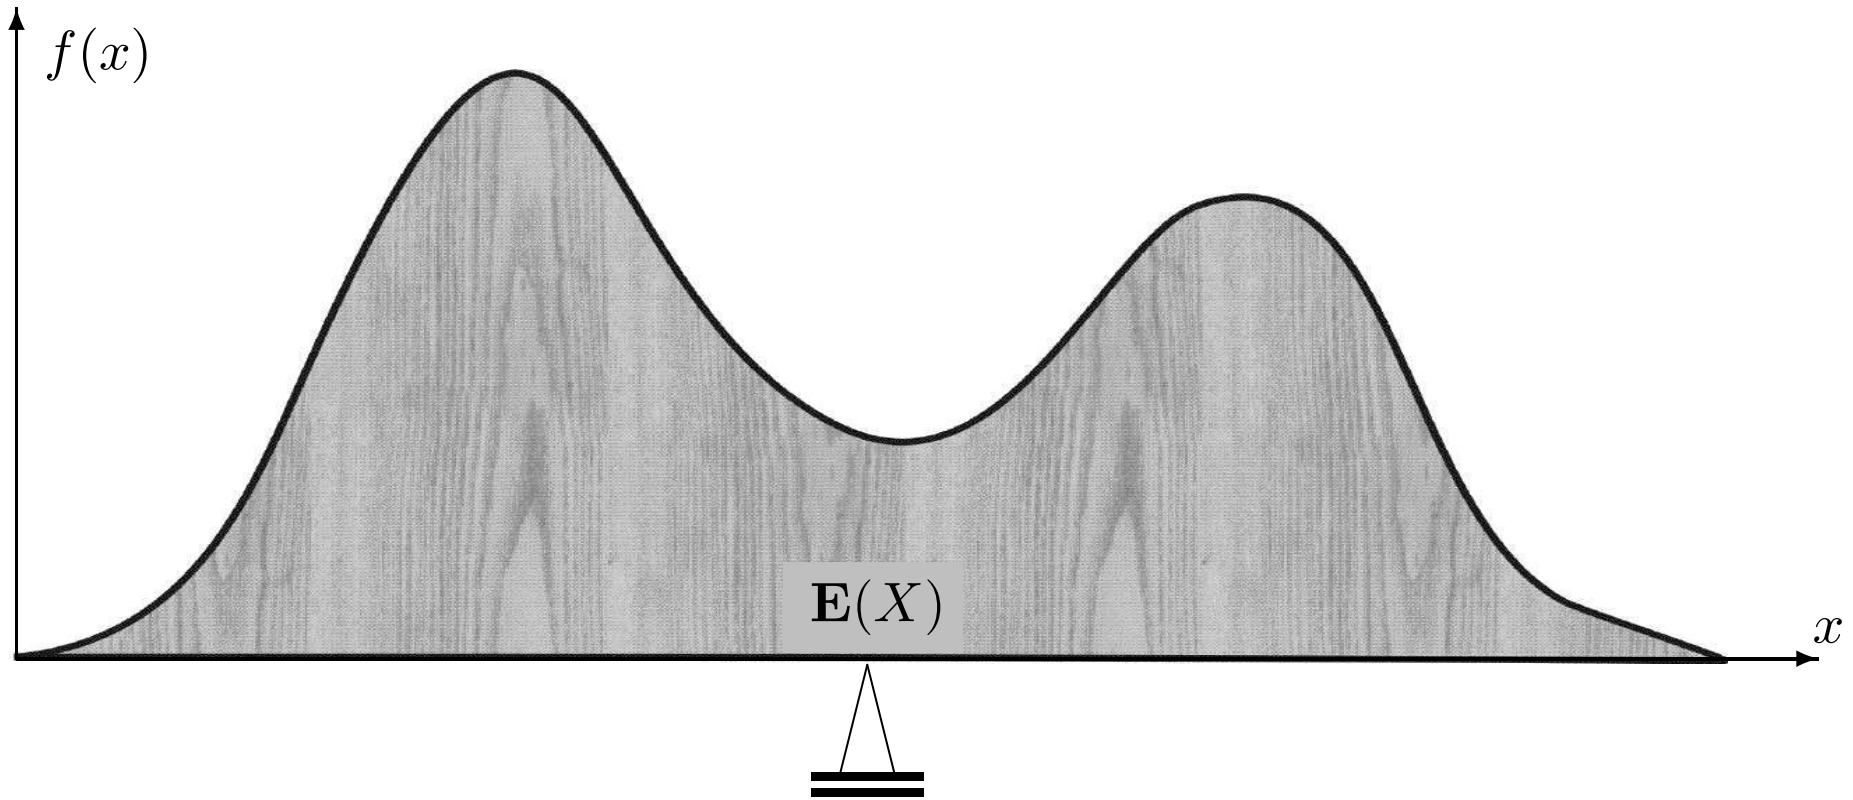
\includegraphics[width=.5\textwidth]{img/Fig4.3.png}
  \caption{\textit{Expectation of a continuous variable as a center of gravity.}}
\end{figure}

\textit{Variance, standard deviation, covariance}, and \textit{correlation} of continuous variables are defined similarly to the discrete case, see Table 3. All the properties in discrete cases extend to the continuous distributions. In calculations, don't forget to replace a pmf with a pdf, and a summation with an integral.

\begin{table}
  \renewcommand{\arraystretch}{2}
  \centering
  \begin{tabular}{|l|l|} 
  \hline
  \textbf{Discrete}                                   & \textbf{Continuous}                                  \\ 
  \hline
  $\begin{aligned}\mathbf{E}(X) = \sum_x xP(x)\end{aligned}$                      & $\begin{aligned}\mathbf{E}(X) = \int xf(x)dx\end{aligned}$                       \\ 
  \hline
  % Second Row
  $\begin{aligned}\text{Var}(X) &= \mathbf{E}(X - \mu)^2\\
                                &= \sum_x (x - \mu)^2 P(x)\\
                                &= \sum_x x^2 P(x) - \mu^2\\
  \end{aligned}$ 
  & 
  $\begin{aligned}\text{Var}(X) &= \mathbf{E}(X - \mu)^2\\
                                &= \int (x - \mu)^2 f(x)dx\\
                                &= \int x^2 f(x)dx - \mu^2    
  \end{aligned}$\\
  \hline

  %Third Row
  $\begin{aligned}\text{Cov}(X, Y) &= \mathbf{E}(X - \mu_X)(Y-\mu_Y)\\
                                   &= \sum_x \sum_y (x - \mu_X)(y - \mu_Y)P(x, y)\\
                                   &= \sum_x \sum_y (xy)P(x, y) - \mu_X \mu_Y
  \end{aligned}$
  &
  $\begin{aligned}\text{Cov}(X, Y) &= \mathbf{E}(X - \mu_X)(Y-\mu_Y)\\
                                   &= \int \int (x - \mu_X)(y - \mu_Y)f(x, y)dxdy\\
                                   &= \int \int (xy)f(x, y)dxdy - \mu_X \mu_Y
  \end{aligned}$\\
  \hline
  \end{tabular}
  \caption{\textit{Moments for discrete and continuous distributions.}}
\end{table}

\begin{example_break}{}
  The lifetime, in years, of some electronic component is a continuous random variable with the density
  \begin{equation*}
    f(x) = \begin{cases}
      \dfrac{k}{x^3} &\textnormal{ for } x \geq 1\\
      0 &\textnormal{ for } x < 1\\
    \end{cases}
  \end{equation*}
  Find $k$, draw a graph of the cdf $F(x)$, and compute the probability for the lifetime to exceed 5 years. Then computer expectation and variance.

  Find $k$ from the condition $\begin{aligned}\int f(x)dx = 1\end{aligned}$:
  \begin{equation*}
    \int_{-\infty}^{+\infty} f(x)dx = \int_1^{+\infty} \frac{k}{x^3} dx = - \frac{k}{2x^2} \Big|_{x = 1}^{+\infty} = \frac{k}{2} = 1
  \end{equation*}
  Hence, $k = 2$. Integrating the density, we get the cdf,
  \begin{equation*}
    F(x) = \int_{-\infty}^x f(y)dy = \int_1^x \frac{2}{y^3} dy -\frac{1}{y^2} \Big|_{y=1}^x = 1 - \frac{1}{x^2}\ \ \ \ \textnormal{for $x > 1$}
  \end{equation*}
  
  Next, compute the probability for the lifetime to exceed 5 years,
  \begin{equation*}
    \prob{X > 5} = 1 - F(5) = 1 - \left(1 - \frac{1}{5^2}\right) = 0.04
  \end{equation*}
  We can also obtain this probability by integrating the density,
  \begin{equation*}
    \prob{X > 5} = \int_5^{+\infty} f(x)dx = \int_5^{+\infty} \frac{2}{x^3}dx = -\frac{1}{x^2} \Big|_{x = 5}^{+\infty} = \frac{1}{25} = 0.04
  \end{equation*}
  
  Its expectation equals
  \begin{equation*}
    \mu = \mathbf{E}(X) = \int x f(x)dx = \int_1^{\infty} 2x^{-2}dx = -2x^{-1} \Big|_1^{\infty} = 2
  \end{equation*}

  Computing its variance, we run into a ``surprise'': This variable does not have a finite variance!
  \begin{equation*}
    \sigma^2 = \text{Var}(X) = \int x^2 f(x)dx - \mu^2 = \int_1^{\infty} 2x^{-1}dx - 4 = 2 \ln x \Big|_1^{\infty} - 4 = +\infty
  \end{equation*}
\end{example_break}


\section{Families of Continuous Distributions}

As in the discrete case, varieties of phenomena can be described by relatively few families of continuous distributions. Here, we shall discuss \textit{\textbf{Uniform, Exponential, Gamma}}, and \textit{\textbf{Normal}} families, adding Student's $t$, Pearson's $\chi^2$, and Fisher's $F$ distributions in later chapters.

\subsection{Uniform Distribution}

\textit{\textbf{Uniform distribution}} plays a unique role in stochastic modeling. A random variable with any thinkable distribution can be generated from a Uniform random variable. Many computer languages and software are equipped with a random number generator that produces Uniform random variables. Users can convert them into variables with desired distributions and use for computer simulation of various events and processes.

Also, Uniform distribution is used in any situation when a value is picked ``at random'' from a given interval; that is, without any preference to lower, higher, or medium values. For example, locations of errors in a program, birthdays throughout a year, and many continuous random variables modulo 1, modulo 0.1, 0.01, etc., are uniformly distributed over their corresponding intervals.

To give equal preference to all values, the Uniform distribution has a \textit{constant density} (Figure 3). On the interval $(a, b)$, its density equals
\begin{equation*}
    f(x) = \frac{1}{b - a},\ \ \ \ a < x < b
\end{equation*}
because the rectangular area below the density graph must equal 1.

\begin{figure}[ht]
    \centering
    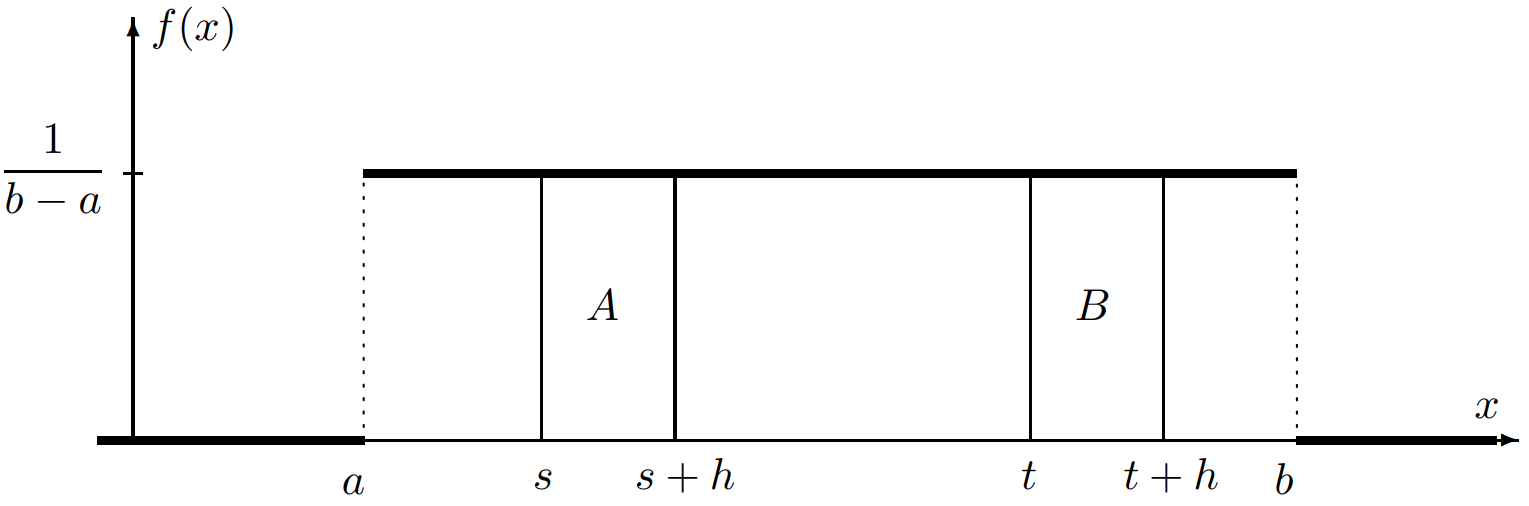
\includegraphics[width=.5\textwidth]{img/Fig4.4.png}
    \caption{\textit{The Uniform density and the Uniform property.}}
\end{figure}

For the same reason, $| b - a |$ has to be a finite number. There does not exist a Uniform distribution on the entire real line. In other words, if you are asked to choose a random number from $(-\infty, +\infty)$, you cannot do it uniformly.

\subsubsection{The Uniform Property}

For any $h > 0$ and $t \in \left[ a, b - h \right]$, the probability
\begin{equation*}
    \prob{t < X < t + h} = \int_t^{t+h} \frac{1}{b - a} dx = \frac{h}{b - a}
\end{equation*}
is \textit{independent} of $t$. This is the \textit{\textbf{Uniform property}}: the probability is only determined by the length of the interval, but not by its location.

\begin{example}{}
In Figure 3, rectangles $A$ and $B$ have the same area, showing that
\begin{equation*}
    \prob{s < X < s + h} = \prob{t < X < t + h}
\end{equation*}
\end{example}

\subsubsection{Standard Uniform Distribution}

The Uniform distribution with $a = 0$ and $b = 1$ is called \textit{Standard Uniform distribution}. The Standard Uniform density is $f(x) = 1$ for $0 < x < 1$. Most random number generators return a Standard Uniform random variable.

All the Uniform distributions are related in the following way. If $X$ is a Uniform$(a, b)$ random variable (\textit{not standard uniform random variable}), then
\begin{equation*}
    Y = \frac{X - a}{b - a}
\end{equation*}
is Standard Uniform \textit{(If X is not inside (0,1), ``X-a'' slides X to the (0,1))}. Likewise, if $Y$ is Standard Uniform, then
\begin{equation*}
    X = a + (b-a)Y
\end{equation*}
is Uniform$(a, b)$. Check that $X \in (a, b)$ if and only if $Y \in (0, 1)$.

A number of other families of distributions have a ``standard'' member. Typically, a simple transformation converts a standard random variable into a non-standard one, and vice versa.

\subsubsection{Expectation and Variance}

For a Standard Uniform variable $Y$,
\begin{equation*}
    \expc{Y} = \int y f(y)dy = \int_0^1 ydy = \frac{1}{2}
\end{equation*}
and
\begin{equation*}
    \var{Y} = \expc{Y^2} - \mathbf{E}^2(Y) = \int_0^1 y^2dy - \left( \frac{1}{2} \right)^2 = \frac{1}{3} - \frac{1}{4} = \frac{1}{12}
\end{equation*}

Now, consider the general case (\textit{Case of not being the standard uniform}). Let $X = a+(b-a)Y$ which has a Uniform$(a, b)$ distribution. By the properties of expectations and variances,
\begin{equation*}
    \expc{X} = \expc{a + (b - a)Y} = a + (b - a)\expc{Y} = a + \frac{b-a}{2} = \frac{a+b}{2}
\end{equation*}
and
\begin{equation*}
    \var{X} =\var{a + (b - a)Y} = (b - a)^2 \var{Y} = \frac{(b - a)^2}{12}
\end{equation*}
The expectation is precisely the middle of the interval $\left[ a, b \right]$. Giving no preference to left or right sides, this agrees with the Uniform property and with the physical meaning of $\expc{X}$ as a center of gravity.

\subsubsection{Uniform Distribution Functions and Variables}
\begin{formula}{Uniform Distribution}
\begin{center}
$\begin{aligned}
    (a, b) &= \text{range of values}\\
    f(x) &= \frac{1}{b - a},\ \ \ \ a < x < b\\
    \expc{X} &= \frac{a+b}{2}\\
    \var{X} &= \frac{(b - a)^2}{12}
\end{aligned}$
\end{center}
\end{formula}

\subsection{Exponential Distribution}

\textbf{\textit{Exponential distribution}} is often used to model \textit{time}: waiting time, interarrival time, hardware lifetime, failure time, time between telephone calls, etc. As we shall see below, in a sequence of rare events, \textit{when the number of events is Poisson, the time between events is Exponential.}

Exponential distribution has density
\begin{equation}
    f(x) = \lambda e^{-\lambda x} \textnormal{ for } x > 0
\end{equation}
With this density, we compute the Exponential cdf, mean, and variance as
\begin{align}
    \prob{X \leq x} = F(x) &= \int_0^x f(t)dt = \int_0^x \lambda e^{-\lambda t} dt = 1 - e^{-\lambda x} \textnormal{    ($x > 0)$}\\
    \expc{X} &= \int tf(t)dt = \int_0^{\infty} t \lambda e^{-\lambda t} = \frac{1}{\lambda} \textnormal{    (integral by parts)}\\
    \var{X} &= \int t^2 f(t)dt - \mathbf{E}^2(X) \nonumber \\
    &= \int_0^{\infty} t^2 \lambda e^{-\lambda t} dt - \left( \frac{1}{\lambda} \right)^2 \textnormal{    (by parts twice)} \nonumber \\
    &= \frac{2}{\lambda^2} - \frac{1}{\lambda^2} = \frac{1}{\lambda^2}
\end{align}
The quantity $\lambda$ is a parameter of Exponential distribution, and its meaning is clear from $\expc{X} = 1/\lambda$. If $X$ is time, measured in minutes, then $\lambda$ is a frequency, measured in min$^{-1}$. For example, if arrivals occur every half a minute, on the average, then $\expc{X} = 0.5$ and $\lambda = 2$, saying that they occur with a frequency (arrival rate) of 2 arrivals per minute. This $\lambda$ has the same meaning as the parameter of Poisson distribution.
\begin{formula}{Important Note}
    \begin{center}
    $\prob{X > x} = 1 - \prob{X \leq x} = 1 - (1 - e^{-\lambda x}) = e^{-\lambda x}$
    \end{center}
    In here $X$ is ``\textit{time between two events}'' and $x$ is ``\textit{particular time}''. So, if this particular time, $x$, is greater than or equal to time between two events, $X$, the eq. 2 is used. Otherwise, the equation inside this box is used.

    \quad ``\textbf{\textit{Exponential distribution}} is a continuous version of \textbf{\textit{Geometric distribution}}. In the \textit{Geometric distribution}, we analyze the how many trials are required before the first success, whereas, in the \textit{Exponential distribution}, we analyze the time until the first success.''
\end{formula}

\subsubsection{Times between rare events are Exponential}

What makes Exponential distribution a good model for interarrival times? Apparently, this is not only experimental, but also a mathematical fact.

As in Chapter 3, consider the sequence of rare events, where the number of occurrences during time $t$ has Poisson distribution with a parameter proportional to $t$. 

Event ``the time $T$ until the next event is greater than $t$'' can be rephrased as ``zero events occur by the time $t$'', and further, as ``$X = 0$'', where $X$ is the number of events during the time interval $\left[ 0, t \right]$ (\textit{It is related with the note in previous page}). This $X$ has Poisson distribution with parameter $\lambda t$. It equals 0 with probability
\begin{equation*}
    P_X(0) = e^{-\lambda t} \frac{(\lambda t)^2}{0!} = e^{-\lambda t}
\end{equation*}
Then we can compute the cdf of $T$ as
\begin{equation}
    F_T(t) = 1 - \prob{T > t} = 1 - \prob{X = 0} = 1 - e^{-\lambda t}
\end{equation}
and here we recognize the Exponential cdf. Therefore, the time until the next arrival has Exponential distribution.

\begin{example}{}
Jobs are sent to a printer at an average rate of 3 jobs per hour.

(a) What is the expected time between jobs?
(b) What is the probability that the next job is sent within 5 minutes?

\textbf{Solution:}
Job arrivals represent rare events, thus the time $T$ between them is Exponential with the given parameter $\lambda = 3$ hrs$^{-1}$ (jobs per hour).

(a) $\expc{T} = 1/\lambda = 1/3$ hours or 20 minutes between jobs.

(b) Convert to the same measurement unit: 5 min = (1/12) hrs. Then,
\begin{equation*}
    \prob{T < 1/12 \textnormal{ hrs}} = F(1/12) = 1 - e^{-\lambda (1/12)} = 1 - e^{1/4} = 0.2212
\end{equation*}
\end{example}

\subsubsection{Memoryless Property}

It is said that ``Exponential variables lose memory''. What does it mean?

Suppose that an Exponential variable $T$ represents waiting time. Memoryless property means that the fact of having waited for $t$ minutes gets ``\textit{forgotten}'', and it \textit{does not affect the future waiting time}. Regardless of the event $T > t$, when the total waiting time exceeds $t$, the remaining waiting time still has Exponential distribution with the same parameter. Mathematically,
\begin{equation}
    \prob{T > t + x\ |\ T > t} = \prob{T > x}\ \ \ \ \textnormal{ for } t, x > 0
\end{equation}
In this formula, $t$ is the already elapsed portion of waiting time, and $x$ is the additional, remaining time.
\begin{proof}
    $\prob{T > x} = e^{-\lambda x}$. Also, by the formula for conditional probability,
    \begin{equation*}
        \prob{T > t + x\ |\ T > t} = \frac{\prob{T > t + x \cap T > t}}{\prob{T > t}} = \frac{\prob{T > t + x}}{\prob{T > t}} = \frac{e^{-\lambda (t+x)}}{e^{-\lambda t}} = e^{-\lambda x}
    \end{equation*}
\end{proof}
This property is unique for Exponential distribution. No other continuous variable $X \in (0, \infty)$ is memoryless. Among discrete variables, such a property belongs to Geometric distribution.

\subsubsection{Exponential Distribution Functions and Variables}

\begin{formula}{Exponential Distribution}
\begin{center}
    $\begin{aligned}
        \lambda &= \textnormal{frequency parameter, the number of events
        per time unit}\\
        f(x) &= \lambda e^{-\lambda x},\ \ \ \ x > 0\\
        \expc{X} &= \frac{1}{\lambda}\\
        \var{X} &= \frac{1}{\lambda^2}
    \end{aligned}$
\end{center}
\end{formula}

\subsection{Gamma Distributinon}

When a certain procedure consists of $\alpha$ independent steps, and each step takes Exponential($\lambda$) amount of time, then the total time has \textit{\textbf{Gamma distribution}} with parameters $\alpha$ and $\lambda$.

Thus, Gamma distribution can be widely used for the total time of a multistage scheme, for example, \textit{related to downloading or installing a number of files}. In a process of rare events, with Exponential times between any two consecutive events, the time of the $\alpha$-th event has Gamma distribution because it consists of $\alpha$ independent Exponential times.

\begin{example}{: Internet Promotions}
    Users visit a certain internet site at the average rate of 12 hits per minute. Every sixth visitor receives some promotion that comes in a form of a flashing banner. Then the time between consecutive promotions has Gamma distribution with parameters $\alpha = 6$ and $\lambda = 12$. 
\end{example}

Having two parameters, Gamma distribution family offers a variety of models for positive random variables. Besides the case when \underline{\textit{a Gamma variable represents a sum of independent Exponential variables}}, Gamma distribution is often used for \textit{the amount of money being paid, amount of a commodity being used (gas, electricity, etc.), a loss incurred by some accident}, etc.

Gamma distribution has a density
\begin{equation}
    f(x) = \frac{\lambda^{\alpha}}{\Gamma(\alpha)} x^{\alpha-1}e^{-\lambda x},\ \ \ \ x > 0
\end{equation}

The denominator contains a Gamma function, later. With certain techniques, this density can be mathematically derived for integer $\alpha$ by representing a Gamma variable $X$ as a sum of Exponential variables each having a density (eq. 1).

In fact, $\alpha$ can take \textit{any positive value}, not necessarily integer. With different $\alpha$, the Gamma density takes different shapes (Figure 4.5). For this reason, $\alpha$ is called a \textit{shape parameter}.

\begin{figure}[h!]
    \centering
    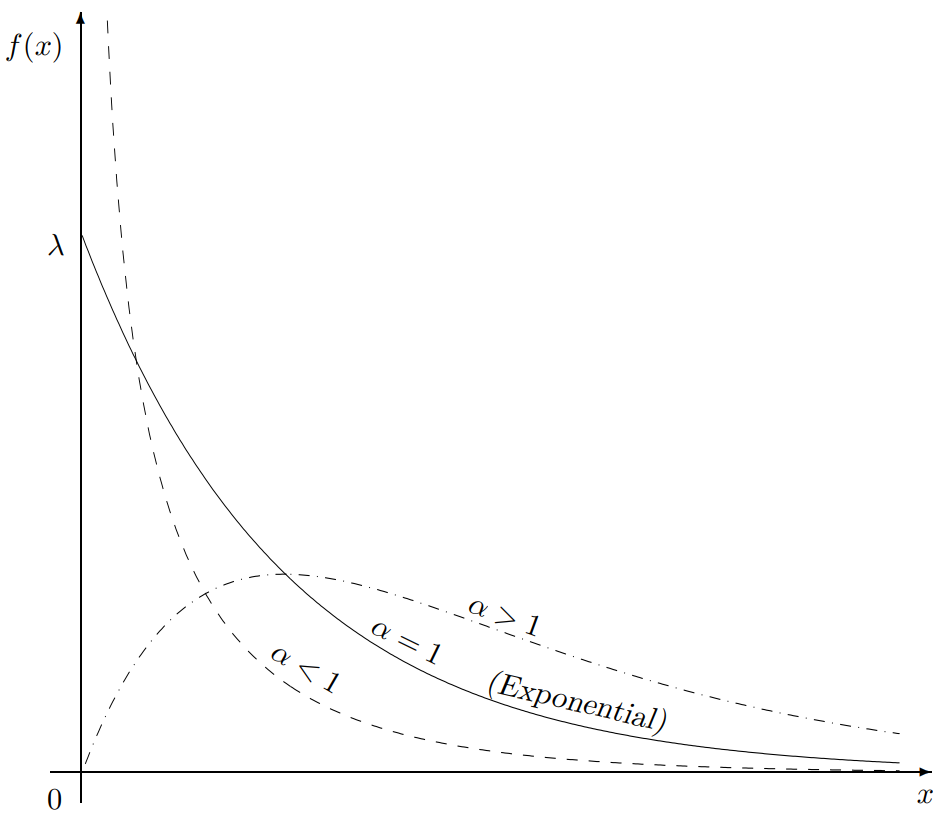
\includegraphics[width=.35\textwidth]{img/Fig4.5.png}
    \caption{\textit{Gamma densities with different shape parameters $\alpha$.}}
\end{figure}

Notice two important special cases of a Gamma distribution. When $\alpha = 1$, the Gamma distribution becomes Exponential. This can be seen comparing (eq. 7) and (eq. 1) for $\alpha = 1$. Another special case with $\lambda = 1/2$ and any $\alpha > 0$ results in a so-called \textit{Chi-square distribution} with ($2\alpha$) degrees of freedom.

\begin{formula}{Special Cases}
    \begin{center}
        $\begin{aligned}
            \textnormal{Gamma}(1, \lambda) &= \textnormal{Exponential}(\lambda)\\
            \textnormal{Gamma}(\alpha, 1/2) &= \textnormal{Chi-square}(2\alpha)\\
        \end{aligned}$
    \end{center}
\end{formula}

\subsubsection{Expectation, Variance, and some useful integration remarks}

Gamma cdf has the form
\begin{equation}
    F(t) = \int_{0}^{t} f(x)dx = \frac{\lambda^{\alpha}}{\Gamma(\alpha)} \int_{0}^{t} x^{\alpha-1} e^{-\lambda x} dx
\end{equation}

This expression, related to a so-called \textit{incomplete Gamma function}, does not simplify, and thus, computing probabilities is not always trivial. Let us offer several computational shortcuts.

First, let us notice that $\begin{aligned}\int_{0}^{\infty} f(x)dx = 1\end{aligned}$ for Gamma and all the other densities. Then, integrating (eq. 7) from $0$ to $\infty$, we obtain that
\begin{equation}
    \int_{0}^{\infty} x^{\alpha-1}e^{-\lambda x} dx = \frac{\Gamma(\alpha)}{\lambda^{\alpha}}\ \ \ \ \textnormal{for any $\alpha > 0$ and $\lambda > 0$}
\end{equation}
Substituting $\alpha + 1$ and $\alpha + 2$ in place of $\alpha$, we get for a Gamma variable $X$
\begin{equation}
    \expc{X} = \int_{}^{} xf(x)dx = \frac{\lambda^{\alpha}}{\Gamma(\alpha)} \int_{0}^{\infty} x^{\alpha} e^{-\lambda x} dx = \frac{\lambda^{\alpha}}{\Gamma(\alpha)} \cdot \frac{\Gamma(\alpha+1)}{\lambda^{\alpha+1}} = \frac{\alpha}{\lambda}
\end{equation}
(using the equality $\Gamma(t + 1) = t \Gamma(t)$ that holds for all t > 0),
\begin{equation*}
    \expc{X^2} = \int_{}^{} x^2f(x)dx = \frac{\lambda^{\alpha}}{\Gamma(\alpha)} \int_{0}^{\infty} x^{\alpha+1} e^{-\lambda x} dx = \frac{\lambda^{\alpha}}{\Gamma(\alpha)} \cdot \frac{\Gamma(\alpha+2)}{\lambda^{\alpha+2}} = \frac{(\alpha + 1) \alpha}{\lambda^2}
\end{equation*}
and therefore,
\begin{equation}
    \var{X} = \expc{X^2} - \expcs{X} = \frac{(\alpha+1)\alpha - \alpha^2}{\lambda^2} = \frac{\alpha}{\lambda^2}
\end{equation}
For $\alpha = 1$, this agrees with (eq. 3) and (eq. 4). Moreover, for any integer $\alpha$, (eq. 10) and (eq. 11) can be obtained directly from (eq. 3) and (eq. 4) by representing a Gamma variable $X$ as a sum of independent Exponential($\lambda$) variables $X_1, ..., X_{\alpha}$,
\begin{align*}
    \expc{X} &= \expc{X_1 + ... + X_{\alpha}} = \expc{X_1} + ... + \expc{X_{\alpha}} = \alpha \left( \frac{1}{\lambda} \right)\\
    \var{X} &= \var{X_1 + ... + X_{\alpha}} = \var{X_1} + ... + \var{X_{\alpha}} = \alpha \left( \frac{1}{\lambda^2} \right)\\
\end{align*}

\subsubsection{Gamma Distribution Functions and Variables}

\begin{formula}{Gamma Distribution: Eq. 12}
\begin{center}
    $\begin{aligned}
        \alpha &= \textnormal{shape parameter}\\
        \lambda &= \textnormal{frequency parameter}\\
        f(x) &= \frac{\lambda^{\alpha}}{\Gamma(\alpha)} x^{\alpha-1} e^{-\lambda x},\ \ \ \ x > 0\\
        \expc{X} &= \frac{\alpha}{\lambda}\\
        \var{X} &= \frac{\alpha}{\lambda^2}
    \end{aligned}$
\end{center}
\end{formula}
\setcounter{equation}{12}

\begin{example_break}{: Total compilation time}
    Compilation of a computer program consists of 3 blocks that are processed sequentially, one after another. Each block takes Exponential time with the mean of 5 minutes, independently of other blocks.\\
    
    (a) Compute the expectation and variance of the total compilation time.
    
    (b) Compute the probability for the entire program to be compiled in less than 12 minutes.\\
    
    \textbf{Solution:} The total time $T$ is a sum of three independent Exponential times, therefore, it has Gamma distribution with $\alpha = 3$. The frequency parameter $\lambda = (1/5)\ min^{-1}$ because the Exponential compilation time of each block has expectation $1/\lambda = 5\ min$. \\

    (a) For a Gamma random variable $T$ with $\alpha = 3$ and $\lambda = 1/5$,
    \begin{align*}
        &\expc{T} = \frac{3}{1/5} = 15\ (min) & \textnormal{and} && \var{T} = \frac{3}{(1/5)^2} = 75\ (min^2)
    \end{align*}

    (b) A direct solution involves two rounds of integration by parts,
    \begin{align}
        \prob{T < 12} &= \int_{0}^{12} f(t)dt = \frac{(1/5)^3}{\Gamma(3)} \int_{0}^{12} t^2 e^{-t/5} dt \nonumber\\
        &= \frac{(1/5)^3}{2!} \left( -5t^2e^{-t/5} \Big|^{t=12}_{t=0} + \int_{0}^{12} 10te^{-t/5}dt \right) \nonumber\\
        &= \frac{(1/125)}{2} \left( -5t^2e^{-t/5} - 50te^{-t/5} \Big|^{t=12}_{t=0} + \int_{0}^{12} 50e^{-t/5}dt \right) \nonumber\\
        &= \frac{1}{250} \left( -5t^2e^{-t/5} - 50te^{-t/5} - 250e^{-t/5}dt \right)\Big|^{t=12}_{t=0} \nonumber\\
        &= 1 - e^{-2.4} - 2.4e^{-2.4} - 2.88 e^{-2.4} = 0.4303
    \end{align}
    A much shorter way is to apply the Gamma-Poisson formula below (example 6).
\end{example_break}

\subsubsection{Gamma-Poisson Formula}

Computation of Gamma probabilities can be significantly simplified by thinking of a Gamma variable as the time between some rare events. In particular, one can avoid lengthy integration by parts, as in Example 5, and use Poisson distribution instead.

Indeed, let $T$ be a Gamma variable with an integer parameter $\alpha$ and some positive $\lambda$. This is a distribution of the time of the $\alpha$-th rare event. Then, the event $\{T > t\}$ means that the
$\alpha$-th rare event occurs after the moment $t$, and therefore, \textit{fewer than $\alpha$ rare events occur before the time $t$}. We see that
\begin{equation*}
    \left\{ T > t \right\} = \left\{ X < \alpha \right\}
\end{equation*}
where $X$ is the number of events that occur before the time $t$. This number of rare events $X$ has Poisson distribution with parameter ($\lambda t$); therefore, the probability
\begin{equation*}
    \prob{T > t} = \prob{X < \alpha}
\end{equation*}
and the probability of a complement
\begin{equation*}
    \prob{T \leq t} = \prob{X \geq \alpha}
\end{equation*}
can both be computed using the Poisson distribution of $X$.

\subsubsection{Gamma-Poisson Formula Functions}

\begin{formula}{Gamma-Poisson Formula: Eq. 14}
    For a Gamma($\alpha, \lambda$) variable $T$ and a Poisson($\lambda t$) variable $X$,
    \begin{align*}
        \prob{T > t} &= \prob{X < \alpha}\\
        \prob{T \leq t} &= \prob{X \geq \alpha}
    \end{align*}
\end{formula}
\setcounter{equation}{14}
\textbf{Remark:} Recall that $\prob{T > t} = \prob{T \geq t}$ and $\prob{T < t} = \prob{T \leq t}$ for a Gamma variable $T$, because it is continuous. Hence, (eq. 14) can also be used for the computation of $\prob{T \geq t}$ and $\prob{T < t}$. Conversely, the probability of $\{X = \alpha\}$ cannot be neglected for the Poisson (discrete!) variable $X$, thus the signs in the right-hand sides of (eq. 14) cannot be altered.

\begin{example}{: Total compilation time, continued}
    Here is an alternative solution to Example 5(b). According to the Gamma-Poisson formula with $\alpha = 3$, $\lambda = 1/5$, and $t = 12$,
    \begin{equation*}
        \prob{T < 12} = \prob{X \geq 3} = 1 - F(2) = 1 - 0.5697 = 0.430
    \end{equation*}
    from Table A3 in book, for the Poisson distribution of $X$ with parameter $\lambda t = 2.4$.\newline

    Furthermore, we notice that the four-term mathematical expression that we obtained in (eq. 13) after integrating by parts represents precisely
    $\prob{X \geq 3} = 1 - P(0) - P(1) - P(2)$.
\end{example}

\begin{example}{}
    Lifetimes of computer memory chips have Gamma distribution with expectation $\mu = 12$ years and standard deviation $\sigma = 4$ years. What is the probability that such a chip has a lifetime between 8 and 10 years?

    \textbf{Solution:} 
    
    \texttt{STEP 1, PARAMETERS}. From the given data, compute parameters of this Gamma distribution. Using (eq. 12), obtain a system of two equations and solve them for $\alpha$ and $\lambda$,
    \begin{center}
        $\begin{cases}
            \mu = \alpha/\lambda\\
            \sigma^2 = \alpha/\lambda^2
        \end{cases}
        \Rightarrow
        \begin{cases}
            \alpha = \mu^2/\sigma^2 = (12/4)^2 = 9\\
            \lambda = \mu/\sigma^2 = 15/4^2 = 0.75
        \end{cases}$
    \end{center}

    \texttt{STEP 2, PROBABILITY}. We can now compute the probability,
    \begin{equation}
        \prob{8 < T < 10} = F_T(10) - F_T(8)
    \end{equation}
    For each term in (eq. 15), we use the Gamma-Poisson formula with $\alpha = 9$, $\lambda = 0.75$, and $t = 8, 10$,
    \begin{equation*}
        F_T(10) = \prob{T \leq 10} = \prob{X \geq 9} = 1 - F_X(8) = 1 - 0.662 = 0.338
    \end{equation*}
    from Table A3 in book, for a Poisson variable $X$ with parameter $\lambda t = (0.75)(10) = 7.5$;
    \begin{equation*}
        F_T(8) = \prob{T \leq 8} = \prob{X \geq 9} = 1 - F_X(8) = 1 - 0.847 = 0.153
    \end{equation*}
    from Table A3 in book, for a Poisson variable $X$ with parameter $\lambda t = (0.75)(8) = 6$. then
    \begin{equation*}
        \prob{8 < T < 10} = 0.338 - 0.153 = 0.185
    \end{equation*}
\end{example}

\subsection{Normal Distribution}

\textit{\textbf{Normal distribution}} plays a vital role in Probability and Statistics, mostly because of the \texttt{Central Limit Theorem}, according to which sums and averages often have approximately Normal distribution. Due to this fact, various fluctuations and measurement errors that consist of accumulated number of small terms appear normally distributed.

Besides sums, averages, and errors, Normal distribution is often found to be a good model for \textit{physical variables like weight, height, temperature, voltage, pollution level, and for instance, household incomes or student grades}.

Normal distribution has a density
\begin{equation*}
    f(x) = \frac{1}{\sigma \sqrt[]{2 \pi}} \textnormal{exp}\left\{ \frac{-(x - \mu)^2}{2\sigma^2} \right\},\ \ \ \ -\infty < x < +\infty
\end{equation*}
where parameters $\mu$ and $\sigma$ have a simple meaning of the expectation $\expc{X}$ and the standard deviation Std($X$). This density is known as the bell-shaped curve, symmetric and centered at $\mu$, its spread being controlled by $\sigma$. As seen in Figure 5, changing $\mu$ shifts the curve to the left or to the right without affecting its shape, while changing $\sigma$ makes it more concentrated or more flat. Often $\mu$ and $\sigma$ are called \textit{location} and \textit{scale} parameters.

\begin{figure}[h!]
    \centering
    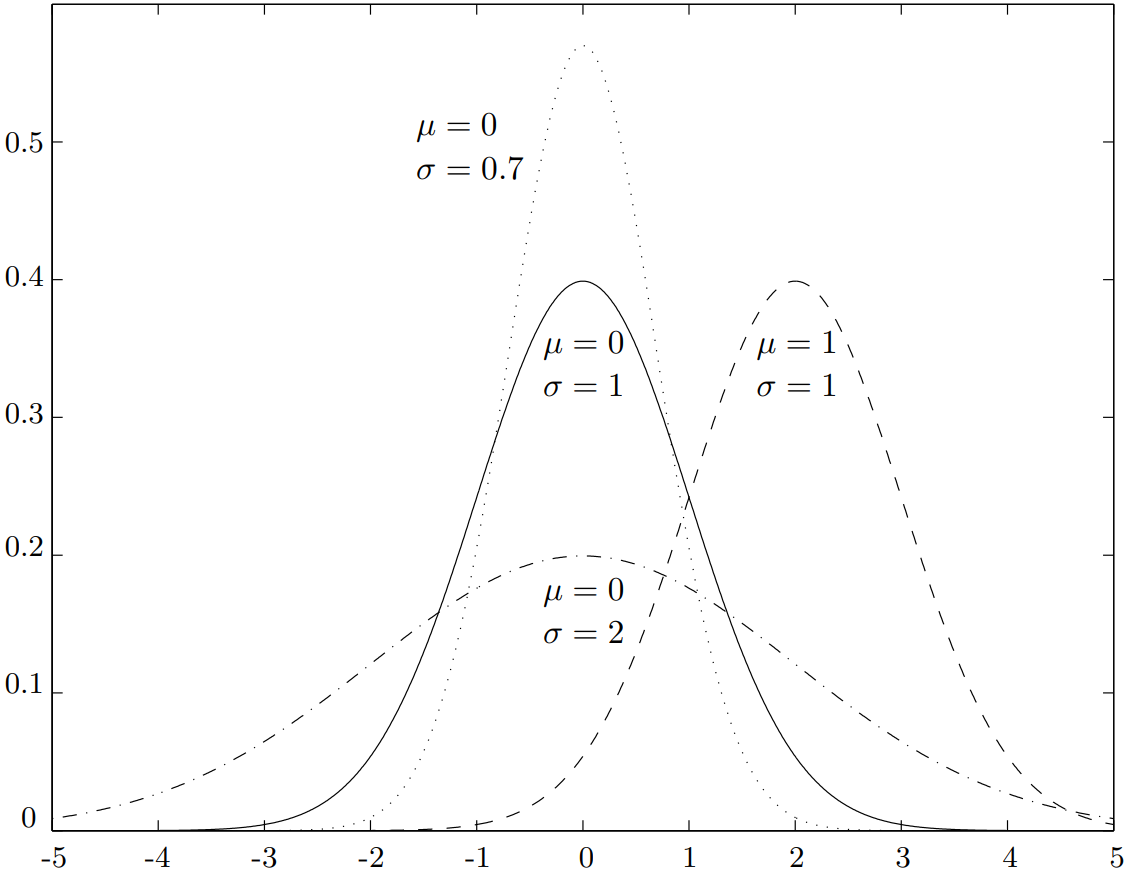
\includegraphics[width=.5\textwidth]{img/Fig4.6.png}
    \caption{\textit{Normal densities with different location and scale parameters.}}
\end{figure}

\subsubsection{Normal Distribution Functions and Variables}

\begin{formula}{}
    \begin{center}
        $\begin{aligned}
            \mu &= \textnormal{expectation, \textit{location} parameter}\\
            \sigma &= \textnormal{standard deviation, \textit{scale} parameter}\\
            f(x) &= \frac{1}{\sigma \sqrt[]{2 \pi}} \textnormal{exp}\left\{ \frac{-(x - \mu)^2}{2\sigma^2} \right\},\ \ \ \ -\infty < x < +\infty\\
            \expc{X} &= \mu\\
            \var{X} &= \sigma^2
        \end{aligned}$
    \end{center}
\end{formula}

\subsubsection{Standard Normal Distribution}

\begin{definition}{}
    Normal distribution with ``standard parameters'' $\mu = 0$ and $\sigma = 1$ is called \textbf{Standard Normal distribution}.
\end{definition}

\begin{formula}{NOTATION}
    \begin{center}
        $\begin{aligned}
            Z &= \textnormal{Standard Normal random variable}\\
            \phi(x) &= \frac{1}{\sqrt[]{2 \pi}} e^{-x^2/2},\textnormal{ Standard Normal pdf}\\
            \Phi(x) &= \int_{-\infty}^{x} \frac{1}{\sqrt[]{2 \pi}} e^{-z^2/2} dz, \textnormal{ Standard Normal cdf}
        \end{aligned}$
    \end{center}
\end{formula}

A Standard Normal variable, usually denoted by $Z$, can be obtained from a non-standard Normal($\mu, \sigma$) random variable $X$ by \textit{standardizing}, that is, subtracting the mean and dividing by the standard deviation,
\begin{equation}
    Z = \frac{X - \mu}{\sigma}
\end{equation}
\textit{Unstandardizing} $Z$, we can reconstruct the initial variable $X$,
\begin{equation}
    X = \mu + \sigma Z
\end{equation}
Using these transformations, any Normal random variable can be obtained from a Standard Normal variable $Z$; therefore, we need a table of Standard Normal Distribution only (Table A4 in book).

\begin{example}{: Computing non-standard Normal probabilities}
    Suppose that the average household income in some country is 900 coins, and the standard deviation is 200 coins. Assuming the Normal distribution of incomes, compute the proportion of ``the middle class'', whose income is between 600 and 1200 coins.

    \textbf{Solution:} Standardize and use Table A4. For a Normal($\mu = 900, \sigma = 200$) variable $X$,
    \begin{align*}
        \prob{600 < X < 1200} &= \prob{\frac{600 - \mu}{\sigma} < \frac{X - \mu}{\sigma} < \frac{1200 - \mu}{\sigma}}\\
        &= \prob{\frac{600 - 900}{200} < Z < \frac{1200-900}{200}} = \prob{-1.5 < Z < 1.5}\\
        &= \Phi(1.5) - \Phi(-1.5) = 0.9332 - 0.0668 = 0.8664
    \end{align*}
\end{example}

So far, we were computing probabilities of clearly defined events. These are direct problems. A number of applications require solution of an inverse problem, that is, finding a value of $x$ given the corresponding probability.

\begin{example_break}{: Inverse problem}
    The government of the country in Example 8 decides to issue food stamps to the poorest 3\% of households. Below what income will families receive food stamps?

    \textbf{Solution:} We need to find such income $x$ that $\prob{X < x} = 3\% = 0.03$. This is an equation that can be solved in terms of $x$. Again, we standardize first, then use the table:
    \begin{equation*}
        \prob{X < x} = \prob{Z < \frac{x - \mu}{\sigma}} = \Phi\left( \frac{x - \mu}{\sigma} \right) = 0.03,
    \end{equation*}
    from where
    \begin{equation*}
        x = \mu + \sigma\Phi^{-1}(0.03)
    \end{equation*}
    In Table A4, we have to find the probability, the table entry of 0.03. We see that $\Phi(-1.88) \approx 0.03$. Therefore, $\Phi^{-1}(0.03) = -1.88$, and
    \begin{equation*}
        x = \mu + \sigma(-1.88) = 900 + (200)(-1.88) = 524\ (coins)
    \end{equation*}
    is the answer. In the literature, the value $\Phi^{-1}(\alpha)$ is often denoted by $z_{1-\alpha}$.
\end{example_break}

As seen in this example, in order to solve an inverse problem, we use the table first, then unstandardize, as in (eq. 17), and find the required value of $x$.


\section{Central Limit Theorem}

We now turn our attention to sums of random variables,
\begin{equation*}
    S_n = X_1 + ... + X_n,
\end{equation*}
that appear in many applications. Let $\mu = \expc{X_i}$ and $\sigma = \textnormal{Std}(X_i)$ for all $i = 1, ..., n$. How does $S_n$ behave for large $n$?

\begin{itemize}
    \item The pure sum $S_n$ diverges. In fact, this should be anticipated because
    \begin{equation*}
        \var{S_n} = n\sigma^2 \rightarrow \infty
    \end{equation*}
    so that variability of $S_n$ grows unboundedly as $n$ goes to infinity.
    \item The average $\dfrac{S_n}{n}$ converges. Indeed, in this case, we have
    \begin{equation*}
        \var{\frac{S_n}{n}} = \frac{\var{S_n}}{n^2} = \frac{n\sigma^2}{n^2} = \frac{\sigma^2}{n} \rightarrow 0
    \end{equation*}
    so that variability of $\dfrac{S_n}{n}$ vanishes as $n \to \infty$.
    \item An interesting normalization factor is $\dfrac{1}{\sqrt[]{n}}$. For $\mu = 0$, $\dfrac{S_n}{\sqrt{n}}$ \textit{neither diverges nor converges}! It does not tend to leave 0, but it does not converge to 0 either. Rather, it behaves like some random variable. The following theorem states that this variable has approximately Normal distribution for large $n$.
\end{itemize}

\begin{theorem}{: Central Limit Theorem}
    Let $X_1, X_2, ...$ be independent random variables with the same expectation $\mu = \expc{X_i}$ and the same standard deviation $\sigma = \textnormal{Std}(X_i)$, and let
    \begin{equation*}
        S_n = \sum_{i=1}^{n} X_i = X_i + ... + X_n
    \end{equation*}
    As $n \to \infty$, the standardized sum
    \begin{equation*}
        Z_n = \frac{S_n - \expc{S_n}}{\textnormal{Std}(S_n)} = \frac{S_n - n\mu}{\sigma\sqrt{n}}
    \end{equation*}
    converges in distribution to a Standard Normal random variable, that is,
    \begin{equation}
        F_{Z_n}(z) = \prob{\frac{S_n-n\mu}{\sigma\sqrt{n}} \leq z} \to \Phi(z)
    \end{equation}
    for all $z$.
\end{theorem}

This theorem is very powerful because it can be applied to random variables $X_1, X_2, ...$ having virtually any thinkable distribution with finite expectation and variance. As long as $n$ is large (the rule of thumb is $n > 30$), one can use Normal distribution to compute probabilities about $S_n$.

Theorem 1 is only one basic version of the \texttt{Central Limit Theorem}. Over the last two centuries, it has been extended to large classes of dependent variables and vectors, stochastic processes, and so on.

\begin{example}{: Allocation of disk space}
    A disk has free space of 330 megabytes. Is it likely to be sufficient for 300 independent images, if each image has expected size of 1 megabyte with a standard deviation of 0.5 megabytes?\\

    \textbf{Solution:} We have $n = 300$, $\mu = 1$, $\sigma = 0.5$. The number of images $n$ is large, so the Central Limit Theorem applies to their total size $S_n$. Then,
    \begin{align*}
        \prob{\textnormal{sufficient space}} &= \prob{S_n \leq 330} = \prob{\frac{S_n - n\mu}{\sigma \sqrt{n}} \leq \frac{330-(300)(1)}{0.5\sqrt{300}}}\\
        &\approx \Phi(3.46) = 0.9997
    \end{align*}
    This probability is very high, hence, the available disk space is very likely to be sufficient.
\end{example}

In the special case of Normal variables $X_1, X_2, ...$, the distribution of $S_n$ is always Normal, and (eq. 18) becomes exact equality for arbitrary, even small $n$.

\begin{example}{: Elevator}
    You wait for an elevator, whose capacity is 2000 pounds. The elevator comes with ten adult passengers. Suppose your own weight is 150 lbs, and you heard that human weights are normally distributed with the mean of 165 lbs and the standard deviation of 20 lbs. Would you board this elevator or wait for the next one?\\

    \textbf{Solution:}
    In other words, is overload likely? The probability of an overload equals 
    \begin{align*}
        \prob{S_{10} + 150 > 2000} &= \prob{\frac{S_10-(10)(165)}{20\sqrt{10}} > \frac{2000-150-(10)(165)}{20\sqrt{10}}}\\
        &= 1 - \Phi(3.16) = 0.0008
    \end{align*}
    So, with probability 0.9992 it is safe to take this elevator. It is now for you to decide.
\end{example}

Among the random variables discussed in Chapters 3 and 4, at least three have a form of $S_n$:
\begin{align*}
    &\textnormal{Binomial variable} &= &&&\textnormal{sum of independent Bernoulli variables}\\
    &\textnormal{Negative Binomial variable} &= &&&\textnormal{sum of independent Geometric variables}\\
    &\textnormal{Gamma variable} &= &&&\textnormal{sum of independent Exponential variables}
\end{align*}
Hence, the Central Limit Theorem applies to all these distributions with sufficiently large $n$ in the case of Binomial, $k$ for Negative Binomial, and $\alpha$ for Gamma variables.

\subsection{Normal Approximation to Binomial Distribution}

Binomial variables represent a special case of $S_n = X_1 + ... + X_n$, where all $X_i$ have Bernoulli distribution with some parameter $p$. We know that small $p$ allows to approximate Binomial distribution with Poisson, and large $p$ allows such an approximation for the number of failures. For the moderate values of $p$ (say, $0.05 \leq p \leq 0.95$) and for large $n$, we can use Theorem 1:
\begin{equation}
    \textnormal{Binomial}(n, p) \approx Normal \left( \mu = np, \sigma = \sqrt{np(1-p)} \right)
\end{equation}

\subsection{Continuity Correction}

This correction is needed when we approximate a discrete distribution (Binomial in this case) by a continuous distribution (Normal). Recall that the probability $\prob{X = x}$ may be positive if $X$ is discrete, whereas it is always 0 for continuous $X$. Thus, a direct use of (eq. 19) will always approximate this probability by 0. It is obviously a poor approximation.

This is resolved by introducing a \textbf{\textit{continuity correction}}. Expand the interval by 0.5 units in each direction, then use the Normal approximation. Notice that
\begin{equation*}
    P_X(x) = \prob{X = x} = \prob{x - 0.5 < X < x + 0.5}
\end{equation*}
is true for a Binomial variable $X$; therefore, the continuity correction does not change the event and preserves its probability. It makes a difference for the Normal distribution, so every time when we approximate some discrete distribution with some continuous distribution, we should be using a continuity correction. Now it is the probability of an interval instead of one number, and it is not zero.

\begin{example}{}
    A new computer virus attacks a folder consisting of 200 files. Each file gets damaged with probability 0.2 independently of other files. What is the probability that fewer than 50 files get damaged?\\

    \textbf{Solution:} The number $X$ of damaged files has Binomial distribution with $n = 200$, $p = 0.2$, $\mu = np = 40$, and $\sigma = \sqrt{np(1-p)} = 5.657$. Applying the Central Limit Theorem with the continuity correction,
    \begin{align*}
        \prob{X < 50} &= \prob{X < 49.5} = \prob{\frac{X-40}{5.657} < \frac{49.5-40}{5.657}}\\
        &= \Phi(1.68) = 0.9535
    \end{align*}
    Notice that the properly applied continuity correction replaces 50 with 49.5, not 50.5. Indeed, we are interested in the event that $X$ is strictly less than 50. This includes all values up to 49 and corresponds to the interval $\left[ 0, 49 \right]$ that we expand to $\left[ 0, 49.5 \right]$. In other words, events $\{X < 50\}$ and $\{X < 49.5\}$ are the same; they include the same possible values of $X$. Events $\{X < 50\}$ and $\{X < 50.5\}$ are different because the former includes $X = 50$, and the latter does not. Replacing $\{X < 50\}$ with $\{X < 50.5\}$ would have changed its probability and would have given a wrong answer.
\end{example}

When a continuous distribution (say, Gamma) is approximated by another continuous distribution (Normal), the continuity correction is not needed. In fact, it would be an error to use it in this case because it would no longer preserve the probability.



\section{Summary and Conclusion}

\begin{itemize}
    \item Continuous distributions are used to model various times, sizes, measurements, and all other random variables that assume an entire interval of possible values.
    \item Continuous distributions are described by their densities that play a role analogous to probability mass functions of discrete variables. Computing probabilities essentially reduces to integrating a density over the given set. Expectations and variances are defined similarly to the discrete case, replacing a probability mass function by a density and summation by integration.
    \item In different situations, one uses Uniform, Exponential, Gamma, or Normal distributions.
    \item The Central Limit Theorem states that a standardized sum of a large number of independent random variables is approximately Normal, thus Table A4 can be used to compute related probabilities. A continuity correction should be used when a discrete distribution is approximated by a continuous distribution.
\end{itemize}

\end{document}

\documentclass{article}
\usepackage[utf8]{inputenc}
\usepackage{geometry}
\usepackage{graphicx}
\usepackage{amsmath}
\usepackage{amsfonts}
\usepackage{amsthm}
\usepackage{amssymb}
\usepackage[most]{tcolorbox}
\usepackage{array}
\usepackage{latexsym}
\usepackage{alltt}
\usepackage{hyperref}
\usepackage{color, colortbl}
\usepackage{float}
\usepackage{pdfpages}
\usepackage{algpseudocode}
\usepackage{multicol}
\usepackage{multirow}
\usepackage{caption}
\usepackage{xparse}
\usepackage{setspace}
\usepackage{enumitem}
\usepackage{pdflscape}
% \usepackage{parskip}
\usepackage{blindtext}
\usepackage{forest}
\usepackage[newfloat]{minted}
\usepackage{booktabs}


\geometry
{
  a4paper,
  left=12mm,
  right=12mm,
  top=12mm,
  bottom=15mm,
}

% mybox
\newtcolorbox{mybox}[3][]
{
  colframe = #2!25,
  colback  = #2!10,
  coltitle = #2!20!black,  
  title    = {#3},
  #1,
}

\definecolor{ex}{rgb}{1.00,0.65,0.00}
\definecolor{bg}{rgb}{0.95,0.95,0.95}
\setminted
{
	mathescape=true,
	xleftmargin=\parindent,
	bgcolor=bg,
	escapeinside=@@
}

\SetupFloatingEnvironment{listing}{name=Code}

\usetikzlibrary{patterns,positioning,fit,arrows,calc,shapes.geometric,shapes.multipart,decorations.pathreplacing}


% New environments that use mybox
\newcounter{example}[section]
\newenvironment{example}[1]{\begin{mybox}[breakable]{ex}{\refstepcounter{example}\textbf{Example \thesection.\theexample #1}}}{\end{mybox}}

\newcounter{definition}[section]
\newenvironment{definition}[1]{\refstepcounter{definition}\begin{mybox}[breakable]{blue}{\textbf{Definition \thesection.\thedefinition #1}}}{\end{mybox}}

\newcounter{theorem}[section]
\newenvironment{theorem}[1]{\begin{mybox}{red}{\refstepcounter{theorem}\textbf{Theorem \thesection.\thetheorem #1}}}{\end{mybox}}

\newenvironment{formula}[1]{\begin{mybox}{cyan}{\textbf{#1}}}{\end{mybox}}

% Changing maketitle
\makeatletter         
\renewcommand\maketitle{
{\raggedright % Note the extra {
\begin{center}
{\Large \bfseries \@title}\\[2ex] 
{\large \@author \ - \@date}\\[2ex]
\end{center}}} % Note the extra }
\makeatother

% \onehalfspacing % adjust spacing
\setlength{\parskip}{0.5\baselineskip}

% macros
\newcommand{\prob}[1]{\textbf{\textit{P}}\left\{#1\right\}}
\newcommand{\expc}[1]{\mathbf{E}\left(#1\right)}
\newcommand{\expcs}[1]{\mathbf{E}^2\left(#1\right)}
\newcommand{\var}[1]{\text{Var}\left( #1 \right)}
\newcommand{\ra}{\rightarrow}
\newcommand{\Ra}{\Rightarrow}

\def\circtxt#1{$\mathalpha \bigcirc \mkern-13mu \mathtt #1$}

\NewDocumentCommand{\dsum}{%
    e{^_}
}{%
  {% 
    \displaystyle\sum
    \IfValueT{#1}{^{#1}}
    \IfValueT{#2}{_{#2}}
  }
}%

% maketitle variables
\title{CENG 242 - Chapter 8: Type Systems}
\author{Burak Metehan Tunçel}
\date{May 2022}

\begin{document}

\maketitle

\begin{multicols*}{2}
\setlength{\columnsep}{1.5cm}
\setlength{\columnseprule}{0.2pt}

Older programming languages had very simple type systems that are not suitable for large-scale software development. Therefore, there are more powerful type systems, which were adopted by the modern programming languages.

In a programming language, there are choices for type systems. Design choices for types:
\begin{itemize}
  \item \textit{monomorphic} vs \textit{polymorphic} type system.
  \item Is overloading allowed?
  \item Is coercion(auto type conversion) applied, how?
  \item Do type relations and subtypes exist?
\end{itemize}

\subsection*{Monomorphic and Polymorphic}

\textit{\textbf{Monomorphic types:}} Each value has a single specific type. Functions operate on a single type. \texttt{C} and most languages are
monomorphic.

\noindent \textit{\textbf{Polymorphism:}} A type system allowing different data types handled in a uniform interface:
\begin{itemize}
  \item \textit{\textbf{Ad-hoc polymorphism:}} Also called \textit{overloading}. Functions that can be applied to different types and behave differently.
  \item \textit{\textbf{Inclusion polymorphism:}} Polymorphism based on subtyping relation. Function applies to a type and all subtypes of the
  type (class and all subclasses).
  \item \textit{\textbf{Parametric polymorphism:}} Functions that are general and can operate identically on different types.
\end{itemize}

\section{Inclusion Polymorphism}
\label{sec:inc-polymorp}

\textit{\textbf{Inclusion polymorphism}} is a type system in which a type may have subtypes, which inherit operations from that type. In particular, inclusion polymorphism is a key concept of object-oriented languages, in which a class may have subclasses, which inherit methods from that class.

\subsection{Types and Subtypes}
\label{subsec:types-subtypes}

Recall that a type $T$ is a set of values, equipped with some operations. A \textit{\textbf{subtype}} of $T$ is a subset of the values of $T$, equipped with the same operations as $T$. Every value of the subtype is also a value of type $T$, and therefore may be used in a context where a value of type $T$ is expected.

It is better if the programming language allows us to declare the variable's \textit{subtype}, and thus declare more accurately what values it might take. This makes the program easier to understand, and possibly more efficient.

\vspace*{\fill}
\columnbreak

If the programming language supports subtypes, we cannot uniquely state the subtype of a \textit{value}. For example, the value $2$ is not only in the type \texttt{int} but also in the subtypes \texttt{char} and \texttt{short} in \texttt{C}. However, the language should allow the subtype of each variable to be declared explicitly.

\noindent \textbf{General properties of subtypes:}
\begin{itemize}
  \item A necessary condition for $S$ to be a subtype of $T$ is that every value of $S$ is also a value of $T$, in other
  words $S \subseteq T$. A value known to be in subtype $S$ can then safely be used wherever a value of type $T$ is expected.
  \item The type $T$ is equipped with operations that are applicable to all values of type $T$. Each of these operations will \textit{also be applicable to values of the subtype $S$}. We say that $S$ \textit{\textbf{inherits}} these operations.
\end{itemize}

Suppose that a value known to be of type $T_1$ is computed in a context where a value of type $T_2$ is expected. In such a context we have insisted that $T_1$ must be equivalent to $T_2$. In the \textit{presence of subtypes}, however, we can allow a looser compatibility between types $T_1$ and $T_2$.

$T_1$ is \textit{\textbf{compatible}} with $T_2$ if and only if $T_1$ and $T_2$ have values in common. This implies that $T_1$ is a subtype of $T_2$, or $T_2$ is a subtype of $T_1$, or both $T_1$ and $T_2$ are subtypes of some other type.

If $T_1$ is indeed compatible with $T_2$, there are two possible cases of interest:
\begin{itemize}
  \item $T_1$ is a subtype of $T_2$, so all values of type $T_1$ are values of type $T_2$. In this case, the value of type $T_1$ can be used safely in a context where a value of type $T_2$ is expected; no run-time check is necessary.
  \item $T_1$ is not a subtype of $T_2$, so some (but not all) values of type $T_1$ are values of type $T_2$. In this case, the value of type $T_1$ can be used only after a run-time check to determine whether it is also a value of type $T_2$. This is a kind of run-time type check, but much simpler and more efficient than the full run-time type checks needed by a dynamically typed language.
\end{itemize}


\subsection{Classes and Subclasses}
\label{subsec:class-subclass}

A class $C$ is a \textit{set of objects}, equipped with some
operations (constructors and methods). These methods may be inherited by the \textit{subclasses} of $C$. Any object of a subclass may be used in a context where an object of class $C$ is expected.

Consider a class $C$ and a subclass $S$. Each object of class $C$ has one or more variable components, and is equipped with methods that access the variable components.  Each object of class $S$ inherits all the variable components of objects of class $C$, and may have additional variable components. Each object of class $S$ potentially inherits all the methods of objects of class $C$, and may be equipped with additional methods that access the additional variable components.

Subclasses are \textit{not exactly analogous to subtypes}. The objects of the subclass $S$ may be used wherever objects of class $C$ are expected, but the former objects have additional components, so the set of objects of subclass $S$ is \textit{not a subset} of the objects of $C$.

The methods of the superclass remain applicable to objects of the subclass, although they can be overridden (specialized) to the subclass if necessary. 



\section{Parametric Polymorphism}
\label{sec:param-polymorp}

A \textit{\textbf{monomorphic}} (``single-shaped'') procedure can operate only on arguments of a fixed type. A \textit{\textbf{polymorphic}} (``many-shaped'') procedure can operate uniformly on arguments of a whole family of types.

\noindent \textit{\textbf{Parametric polymorphism}} is a \textit{type system} in which we can write polymorphic procedures. The functional language \texttt{HASKELL} are prominent examples of languages that exhibit parametric polymorphism. 

\subsection{Polymorphic Procedures}
\label{subsec:Polymorp-procedure}

A \textit{\textbf{type variable}} is an identifier that stands for any one of a family of types. In this section we shall write type variables as Greek letters ($\alpha, \beta, \gamma, \ldots$), partly for historical reasons and partly because they are easily recognized. In \texttt{HASKELL} type variables are conventionally written as lowercase Roman

A \textit{\textbf{polytype}} derives a family of similar types. Two examples of polytypes are $\sigma \times \tau$ and $\sigma \times \tau \ra \tau$. A polytype always includes one or more type variables.

The family of types derived by a polytype is obtained by making all possible systematic substitutions of types for type variables. The family of types derived by $\sigma \times \tau \ra \tau$ includes
\begin{itemize}
  \item \texttt{Integer $\times$ Boolean $\ra$ Boolean}
  \item \texttt{String $\times$ String $\ra$ String}
\end{itemize}
It does not include
\begin{itemize}
  \item \texttt{Integer $\times$ Boolean $\ra$ Integer}
  \item \texttt{Integer $\ra$ Integer}
  \item \texttt{Integer $\times$ Integer $\times$ Integer $\ra$ Integer}
\end{itemize}
In other words, each type in the family derived by $\sigma \times \tau \ra \tau$ is the type of a function that accepts a pair of values and returns a result of the same type as the second component of the pair.

\noindent In brief:
\begin{itemize}
  \item Operations are same, but types are different.
  \item Types with type variables: \textit{polytypes}.
  \item Most functional languages are polymorphic.
  \item Object oriented languages provide polymorphism through inheritance, run time binding and generics.
\end{itemize} 


\subsection{Parameterized Types}
\label{subsec:param-types}

A \textit{\textbf{parameterized type}} is a type that takes other type(s) as parameters. For instance, consider array types in \texttt{C}. We can think of \texttt{$\tau$[]} as a parameterized type, which can be specialized to an ordinary type (such as \texttt{char[]}, or \texttt{float[]}, or \texttt{float[][]}) by substituting an actual type for the type variable $\tau$.

All programming languages have built-in parameterized types. For instance, \texttt{C} and \texttt{C++} have \texttt{$\tau$[]} and $\tau^*$. But only a few programming languages, notably \texttt{HASKELL}, allow programmers to define their own parameterized types.

\begin{example}{}
Consider the following HASKELL parameterized type definition:
\mint[bgcolor={}]{haskell}{type Pair @$\tau$@ = (@$\tau$@, @$\tau$@)}
In this definition $\tau$ is a type parameter, denoting an unknown type.
\end{example}

\begin{example}{}
The following \texttt{HASKELL} (recursive) parameterized type definition defines homogeneous lists with elements of type $\tau$:
\mint[bgcolor={}]{haskell}{data List @$\tau$@ = Nil | Cons (@$\tau$@, List @$\tau$@)}
\end{example}

\subsubsection{Polymorphism in \texttt{C++} and \texttt{Java}}
\label{subsubsec:poly-in-cpp-java}

In such languages, inheritence provides subtyping polymorphism. \texttt{C++} \mintinline[bgcolor={}]{cpp}{virtual} methods, and all methods in \texttt{Java} implements \textcolor{blue}{late binding} to improve polymorphism  through inheritence.

Generic abstractions, \texttt{C++} \mintinline[bgcolor={}]{cpp}{template} and \texttt{Java} \textcolor{blue}{generics} provide polymorphic classes and functions.
\begin{listing}[H]

\begin{minted}{cpp}
template <typename T>
void sort(T arr[], int n) {
  // ... your favorite sort algorithm here
}
\end{minted}

\begin{minted}{java}
class Test { 
  //Java requires functions be in a class
  void <T> sort(T[] arr) {
    // ... your favorite sort algorithm here
  }
}
\end{minted}

\caption{}
\label{code:code1}
\end{listing}
\texttt{C++} \textcolor{blue}{templates} use compile time binding. \texttt{Java} \textcolor{blue}{generics} binds at run time.

\vspace*{\fill}
\columnbreak


\subsection{Type Inference}
\label{subsec:type-infer}

\textit{\textbf{Type inference}} is a process by which the type of a declared entity is inferred, where it is not explicitly stated. Some functional programming languages such as \texttt{HASKELL} rely heavily on type inference, to the extent that we rarely need to state types explicitly.

Type inference sometimes yields a monotype, but only where the available clues are strong enough. However, the available clues are not always so strong: the function body might be written entirely in terms of polymorphic functions. Indeed, it is conceivable that the function body might provide no clues at all. 

\noindent In these circumstances, type inference will yield a polytype and finds the \textit{most general type satisfying the constraints}.

Excessive reliance on type inference, however, tends to make large programs difficult to understand. 
\begin{itemize}
  \item A reader might have to study the whole of a program in order to discover the types of its individual functions.
  \item Even the implementer of the program could have trouble understanding it: a slight programming error might cause the compiler to infer different types from the ones intended by the implementer, resulting in obscure error messages.
\end{itemize}
So explicitly declaring types, even if redundant, is good programming practice.

\subsubsection{Inferring Type from Initializers}
\label{subsubsec:infer-type-initializers}

\begin{itemize}
  \item C++11 \mintinline[bgcolor={}]{cpp}{auto} type specifier \textit{gets type from initializer or return expression}.
  \item C++11 \mintinline[bgcolor={}]{cpp}{decltype(varexp)} \textit{gets type same as the variables declared type}.
\begin{listing}[H]

\begin{minted}{cpp}
auto f(int a) {
  // double, function becomes double  
  return a/3.0;
}  
struct P { double x, y;} *pptr;

// double since pptr->x is double
decltype(pptr->x) xval;

// initializer is P typed
auto v = (P)({ 2.0, 4.0});
// f(3) returns double so t is double
auto t = f(3);    
\end{minted}

\caption{}
\label{code:code2}
\end{listing}
  
  \item GCC has \textcolor{cyan}{\texttt{typeof(expr)}}, some other dialects have \textcolor{cyan}{\texttt{\_\_typeof\_\_(expr)}} macro having a similar mechanism in \texttt{C}.
\end{itemize}

\vspace*{\fill}
\columnbreak



\section{Overloading}
\label{sec:overloading}

An identifier is said to be \textit{\textbf{overloaded}} if it denotes two or more distinct procedures in the same scope. In other words, \textit{\textbf{overloading}} is using same identifier for multiple places in same
scope.

Such overloading is acceptable only if every procedure call is unambiguous, i.e., the compiler can uniquely identify the procedure to be called using only type information.

\textit{Polymorphic function: one function that can process multiple types.}

C++ allows overloading of functions and operators.
\begin{listing}[H]
\begin{minted}{cpp}
typedef struct Comp { double x, y; } Complex;
double @\color{orange}mult@(double a, double b) { return a * b; }
Complex @\color{brown}mult@(Complex s, Complex u) {
  Complex t;
  t.x = s.x*u.x - s.y*u.y;
  t.y = s.x*u.y + s.y*u.x;
  return t;
}
Complex a,b; double x,y;
a=@\color{brown}mult@(a,b) ; x=@\color{orange}mult@(y,2.1);
\end{minted}
\caption{}
\label{code:code3}
\end{listing}

We can characterize overloading in terms of the types of the overloaded functions. Suppose that an identifier $F$ denotes both a function $f_1$ of type $S_1 \ra T_1$ and a function $f_2$ of type $S_2 \ra T_2$. (Recall that this covers functions with multiple arguments, since $S_1$ or $S_2$ could be a Cartesian product.) The overloading may be either \textit{context-independent} or \textit{context-dependent}.

In brief, binding is more complicated. Binding is made not only according to name but \textcolor{red}{according to name and type}.

\begin{formula}{}

\noindent Function type: \\

\texttt{
  \tikz [remember picture,overlay] \matrix [anchor=west,rounded corners=2mm,thick,rectangle,draw=green!50!black,ampersand replacement=\&] (condep) 
  {
    \node [rectangle,draw=orange!80!black,thick] (conind) { 
      name : {\em parameters\/}
      }; \&
    \node {
      $\rightarrow$ \em result\/
    };\\};} \\

\noindent \textcolor{blue}{Context dependent overloading}:
  \begin{tikzpicture} [overlay,remember picture] 
    \node (here) {}; \draw [<-,thick,black,green!50!black] (condep.south east) |- (here) ;
  \end{tikzpicture}\\
\quad Overloading based on function name, parameter type and return type.

\noindent \textcolor{blue}{Context independent overloading} : 
  \begin{tikzpicture} [overlay,remember picture] 
    \node (here) {}; \draw [->,thick,black,orange!80!black] (here) -| +(2.8,2.7) -| (conind) ;
  \end{tikzpicture}\\
\quad Overloading based on function name and parameter type. No return type!

\end{formula}

\vspace*{\fill}
\columnbreak

\subsection{Context-dependent Overloading}
\label{subsec:depend-overload}

\textit{\textbf{Context-dependent overloading}} requires only that $S_1$ and $S_2$ are non-equivalent or that $T_1$ and $T_2$ are non-equivalent. If $S_1$ and $S_2$ are non-equivalent, the function to be called can be identified as below (\hyperref[subsec:independ-overload]{context-independent overloading}). If $S_1$ and $S_2$ are equivalent but $T_1$ and $T_2$ are non-equivalent, context must be taken into account to identify the function to be called. Consider the function call ``$F(E)$'', where $E$ is of type $S_1$ (equivalent to $S_2$). If the function call occurs in a context where an expression of type $T_1$ is expected, then $F$ must denote $f_1$; if the function call occurs in a context where an expression of type $T_2$ is expected, then $F$ must denote $f_2$.

For example:
Which type does the expression calling the function expects (context) ?
\begin{listing}[H]

\begin{minted}{cpp}
int f(double a) { ...@\color{orange}\circtxt{1}@ }
int f(int a) { ...@\color{green!50!black}\circtxt{2}@ } 
double f(int a) { ...@\color{violet}\circtxt{3}@ }  
double x,y; 
int a,b;
\end{minted}
\caption{}
\label{code:code4}

\end{listing}

\begin{itemize}[leftmargin=*]
  \item[] \texttt{a=f(x)}; {\color{orange}\circtxt{1}} (x double)
  \item[] \texttt{a=f(x)}; {\color{orange}\circtxt{1}} (x double)
  \item[] \texttt{a=f(a)}; {\color{green!50!black}\circtxt{2}} (a int, assign int)
  \item[] \texttt{x=f(a)}; {\color{violet}\circtxt{3}} (a int, assign double)
  \item[] \texttt{x=2.4+f(a)}; {\color{violet}\circtxt{3}} (a int, mult double)
  \item[] \texttt{a=f(f(x))}; {\color{green!50!black}\circtxt{2}}({\color{orange}\circtxt{1}}) ( x double, f(x):int, assign int)
  \item[] \texttt{a=f(f(a))}; {\color{green!50!black}\circtxt{2}}({\color{green!50!black}\circtxt{2}}) or {\color{orange}\circtxt{1}}({\color{violet}\circtxt{3}}) ???
\end{itemize}
Problem gets more complicated. (even forget about coercion)

Context dependent overloading is more expensive, complex and confusing. Most overloading languages are context independent.

\subsection{Context-independent Overloading}
\label{subsec:independ-overload}

\textit{\textbf{Context-independent overloading}} requires that $S_1$ and $S_2$ are non-equivalent. Consider the function call ``$F(E)$''. If the actual parameter $E$ is of type $S_1$, then $F$ here denotes $f_1$ and the result is of type $T_1$. If $E$ is of type $S_2$, then $F$ here denotes $f_2$ and the result is of type $T_2$. With context-independent overloading, the function to be called is always uniquely identified by the type of the actual parameter.

\begin{formula}{\textcolor{brown}{Careful}}
Overloading is useful only for functions doing same operations. Two functions with different purposes should not be given same names. Confuses programmer and causes errors.
\end{formula}

\vspace*{\fill}
\columnbreak

We must be careful not to confuse the distinct concepts of overloading (which is sometimes called \textit{ad hoc polymorphism}) and \textit{parametric polymorphism}. Overloading means that a small number of separately-defined procedures happen to have the same identifier; these procedures do not necessarily have related types, nor do they necessarily perform similar operations on their arguments. Polymorphism is a property of a single procedure that accepts arguments of a large family of related types; the parametric procedure is defined once and operates uniformly on its arguments, whatever their type.


\section{Type Conversion}
\label{sec:type-conversion}

A \textit{\textbf{type conversion}} is a mapping from the values of one type to corresponding values of a different type.

Programming languages vary, not only in which type conversions they define, but also in whether these type conversions are explicit or implicit.

A \textit{\textbf{cast}} is an \textit{explicit type conversion}. In \texttt{C}, \texttt{C++}, and \texttt{JAVA}, a cast has the form ``$(T)E$''. If the subexpression $E$ is of type $S$ (not equivalent to $T$), and if the programming language defines a type conversion from $S$ to $T$, then the cast maps the value of $E$ to the corresponding value of type $T$.

A \textit{\textbf{coercion}} is an implicit type conversion, and is performed automatically wherever the syntactic context demands it. Consider an expression $E$ in a context where a value of type $T$ is expected. If $E$ is of type $S$ (not equivalent to $T$), and if the programming language allows a coercion from $S$ to $T$ in this context, then the coercion maps the value of $E$ to the corresponding value of type $T$.

Some programming languages are very permissive in respect of coercions. However, the general trend in modern programming languages is to minimize or even eliminate coercions altogether, while retaining casts. At first sight this might appear to be a retrograde (back) step. However, coercions fit badly with parametric polymorphism and overloading, concepts that are certainly more useful than coercions. Casts fit well with any type system, and anyway are more general than coercions.


\end{multicols*}

\end{document}


\end{document}
